\documentclass[dvipsnames]{article}
\usepackage[utf8]{inputenc}
\usepackage[left=3cm, right=3cm, top=2cm]{geometry}
\title{Dynamic Boundary Conditions}
\author{Silvin Willemsen}
\date{June 2020}

\usepackage{natbib}
\usepackage{graphicx}
\usepackage{appendix}
\usepackage{amsmath}
\makeatletter
\renewcommand*\env@matrix[1][*\c@MaxMatrixCols c]{%
  \hskip -\arraycolsep
  \let\@ifnextchar\new@ifnextchar
  \array{#1}}
\makeatother

\usepackage{amsfonts}
\usepackage{amssymb}
\usepackage{subfig}
\usepackage{mathtools}
\usepackage{xcolor} 
\usepackage{cases}
\def\SBcomment[#1]{\textcolor{red}{#1}}
\def\SWcomment[#1]{\textcolor{blue}{#1}}
\def\SScomment[#1]{\textcolor{green}{#1}}

\def\type[#1]{\textcolor{purple}{#1}}
\def\mystrut{\rule[-.2\baselineskip]{0pt}{\baselineskip}}

\def\u{\mathbf{u}}
\def\w{\mathbf{w}}
\def\I{\mathbf{I}}
\def\A{\mathbf{A}}
\def\B{\mathbf{B}}
\def\C{\mathbf{C}}
\def\Q{\mathbf{Q}}
\def\U{\mathbf{U}}
\def\J{\mathbf{J}}
\def\Iterm{\mathcal{A}}

\def\Dxx{\mathbf{D}_{xx}}


\begin{document}
\maketitle

\section{Introduction}
This document shows the work done and documentation on dynamic boundary conditions.
 
\section{Motivation}
Let's take the 1D wave equation in discrete time (see Figure \ref{fig:fullString} as an example):
\begin{equation}\label{eq:1Dwave}
    \rho A\delta_{tt}u_l^n=T\delta_{xx}u_l^n,
\end{equation}
parameterised using material density $\rho$, cross-sectional area $A$ and tension $T$, and with simply supported boundary conditions such that
\begin{equation}\label{eq:boundaryCondition}
u_l^n = \delta_{xx}u_l^n = 0 \quad \text{at} \quad l = 0, N,
\end{equation}
which states that both the state of the boundaries and the curvature at the boundaries should be 0. If we expand \eqref{eq:boundaryCondition} at, say, the left boundary, we can introduce a virtual grid point $u_{-1}$ that (as we will see later on) needs to be exactly $-u_1$ to satisfy this condition (see Figures \ref{fig:leftBoundary} and \ref{fig:boundaryCondition}).

Through stability analysis one can arrive at a condition for the grid spacing that needs to be satisfied in order for the implementation to be stable. In this case this is
\begin{equation}\label{eq:stabilityCondition}
    h \geq ck,
\end{equation}
where grid spacing $h$ is the distance between two neighbouring points, wave speed $c = \sqrt{T/\rho A}$ and time step $k = 1/f_\text{s}$ with sample rate $f_\text{s}$. The closer $h$ is to this condition, the more accurate the scheme will be and the less bandwidth we lose. The reason we can't always satisfy condition \eqref{eq:stabilityCondition} with equality (and consequently utilise the full bandwidth) is due to the fact that we require an integer number of grid points. In other words, we can't use ``fractional grid points". Usually, the following steps are followed to calculate $h$ \cite[Section 6.2.10]{Bilbao2009}:
\begin{equation}
    \qquad N := \text{floor}(1/ck) \qquad h := 1/N.
\end{equation}
There are cases where we can satisfy condition \eqref{eq:stabilityCondition} with equality, i.e., when $1/ck$ is an integer ($1/ck = \text{floor}(1/ck)$). For example, when using a wave speed of $c = 1470$ m/s and sample rate $f_\text{s} = 44100$ Hz we can satisfy the stability condition with equality $h = 1/30$ (see Figure \ref{fig:fullString}). However, this is a special case, and if we want to change the wave speed dynamically we need to come up with something smarter. I would like to propose, \textit{interpolated boundary conditions}, the possibility of which has briefly been mentioned by Stefan Bilbao in a footnote \cite[p. 145]{Bilbao2009}, but never elaborated on\footnote{...as ``Footnotes are usually written by people who are pretending to know something but actually don't!" -- Bilbao, 2020.}. 
\begin{figure}[h]
    \centering
    \subfloat[String $N=30$ (or $31$?).]{\label{fig:fullString}{ 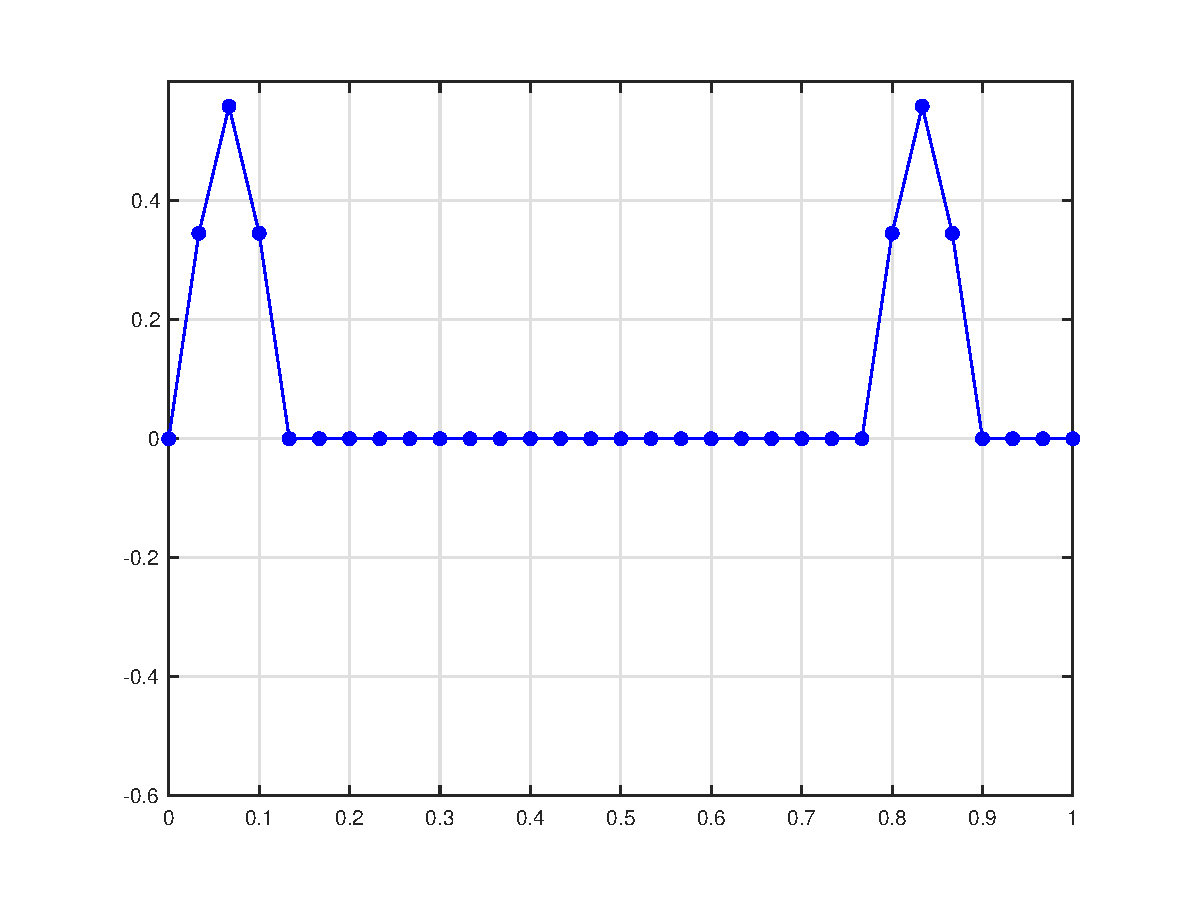
\includegraphics[width=0.33\textwidth]{plot1.eps}}}
    \subfloat[At the left boundary.]{\label{fig:leftBoundary}{ 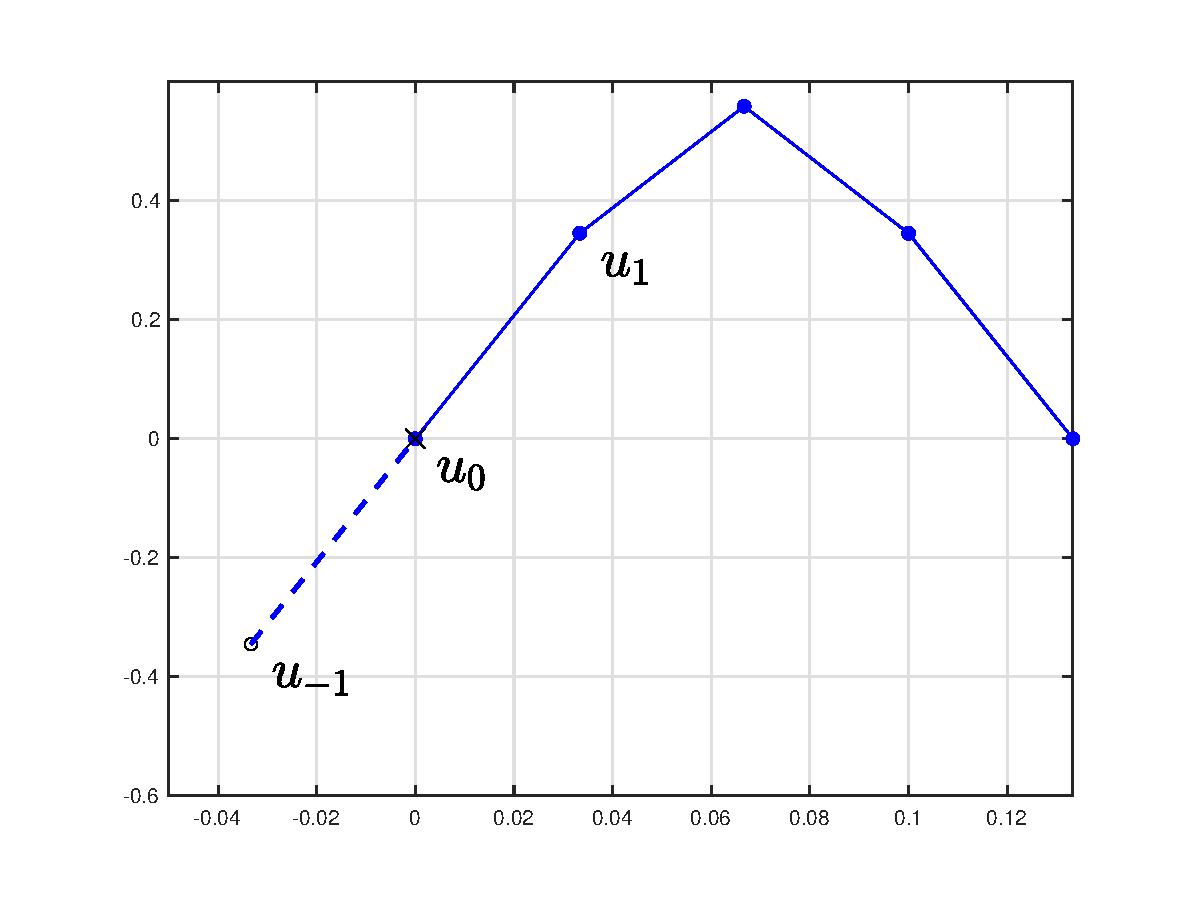
\includegraphics[width=0.33\textwidth]{plot2.eps}}}
    \subfloat[Curvature at the boundary (in this case at $u_0$) should be 0.]{\label{fig:boundaryCondition}{ 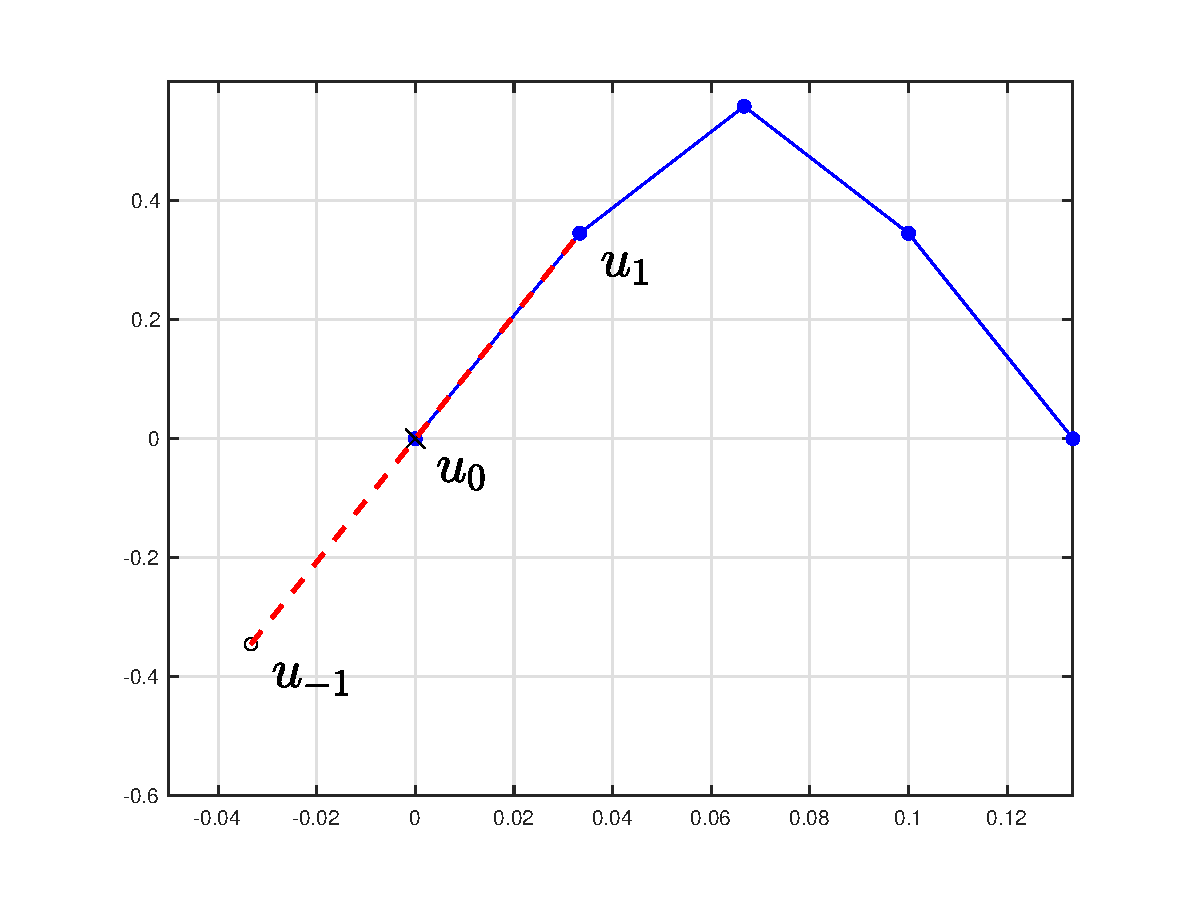
\includegraphics[width=0.33\textwidth]{plot3.eps}}}
    \caption{Case of grid point on boundary.}
\end{figure}

\begin{figure}[h]
\centerline{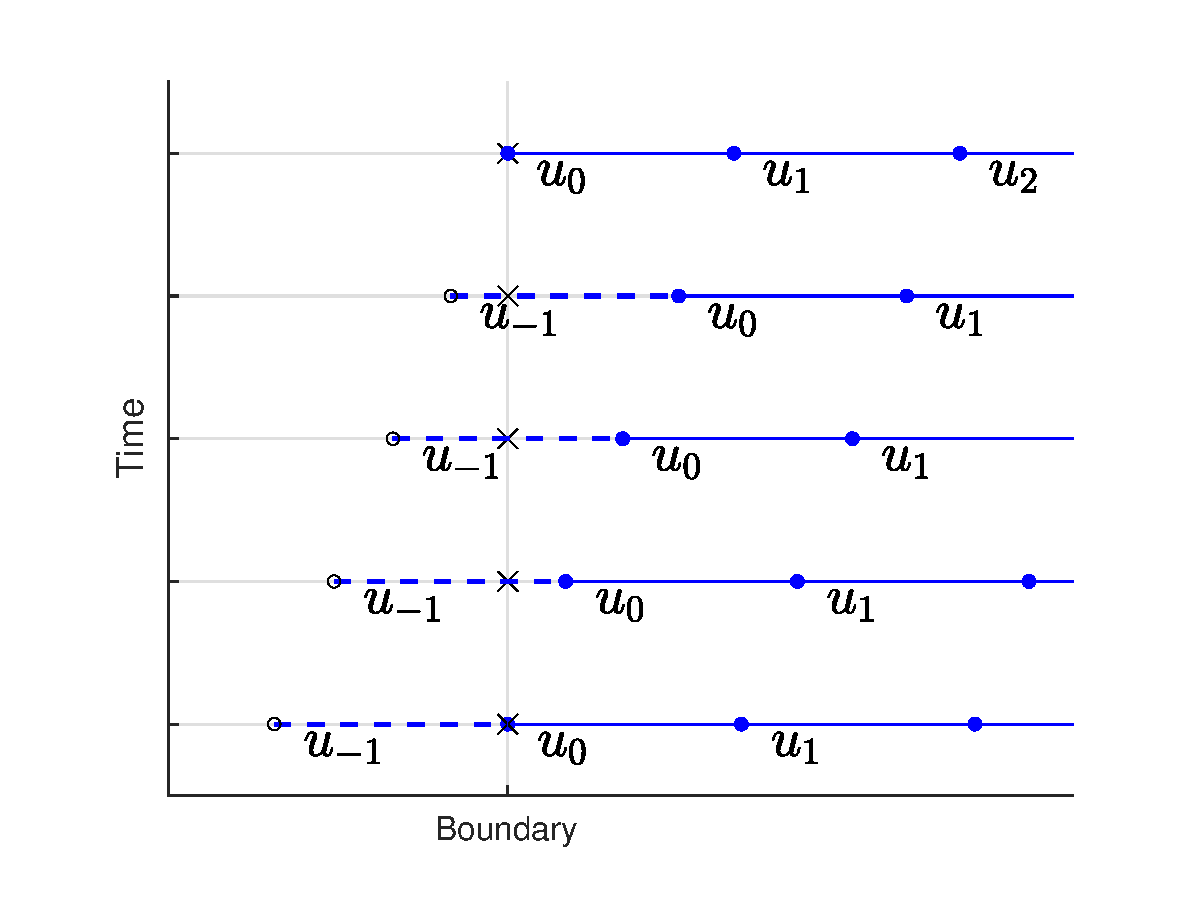
\includegraphics[width=0.6\columnwidth]{dynamic2.eps} }
\caption{\label{fig:dynamicGrid}{Grid changing over time.}}
\end{figure}

\subsection{Analogy with a real-life string}
Imagine detuning a real-life string by turning the tuning knob, we essentially change the value for tension $T$ in Eq. \eqref{eq:1Dwave}. If we imagine the tuning knob being at the nut (left boundary), more material will appear on that side when $T$ decreases, and vice versa. To make the transition to the finite-difference setting easier, imagine equidistant points drawn on this string in such a way that there is a point exactly at the nut and the bridge (i.e. at each boundary). Then, when decreasing the tension, the point at the nut will start moving towards the bridge. As a matter of fact, all points (except for the one at the bridge) will start moving towards the bridge! Effectively, we slowly decrease the space between the points which -- in a finite-difference setting -- is analogous to decreasing the grid spacing $h$ (see Figure \ref{fig:dynamicGrid} with time going from bottom to top). If we do this according to condition \eqref{eq:stabilityCondition}, we get the great side-effect of always satisfying this condition with equality, which means that we don't lose accuracy (or bandwidth). The issue left to solve now is to figure out what to do around the boundary. We continue by keeping in mind boundary condition \eqref{eq:boundaryCondition}.
% \begin{figure}[h]
% \centerline{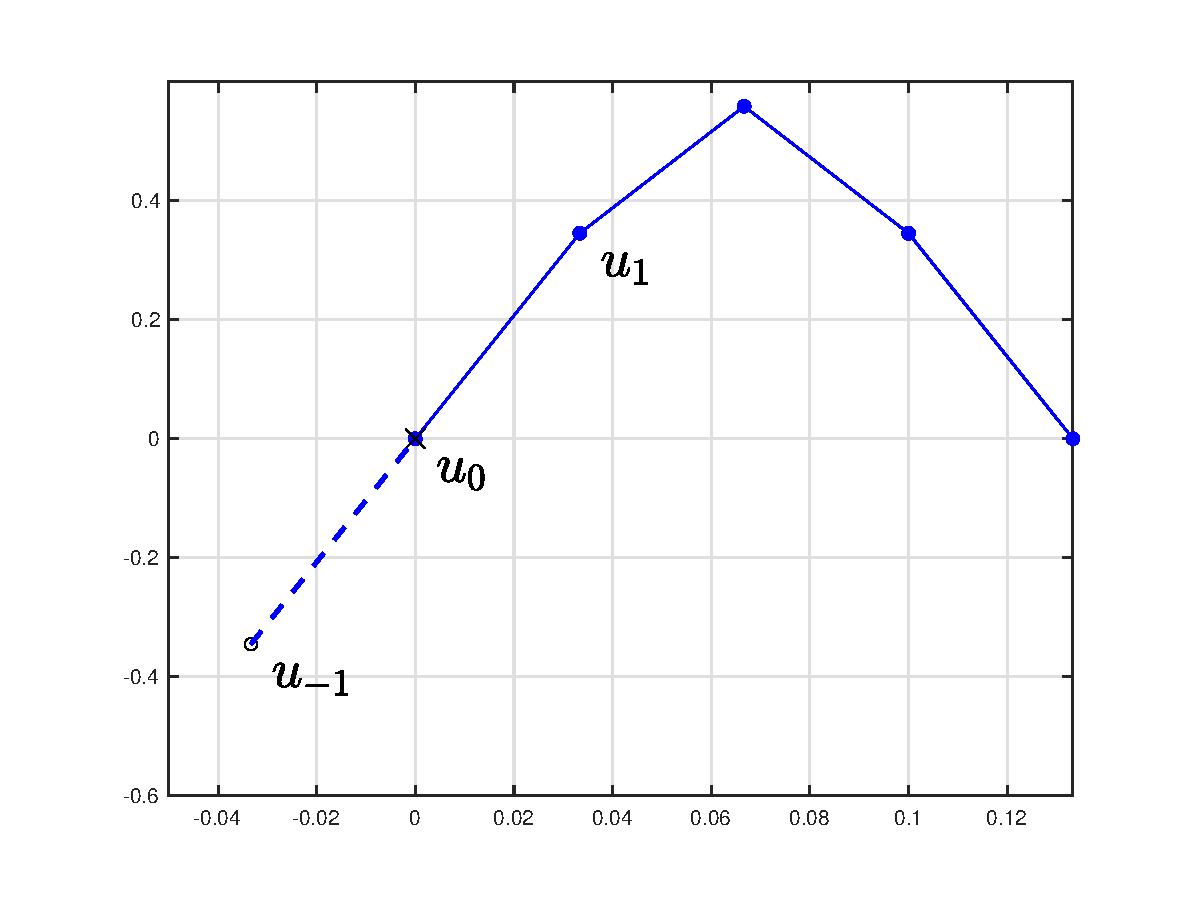
\includegraphics[width=0.6\columnwidth]{plot2.eps}}
% \caption{\label{fig:eta}{At the left boundary.}}
% \end{figure}

% \begin{figure}[h]
% \centerline{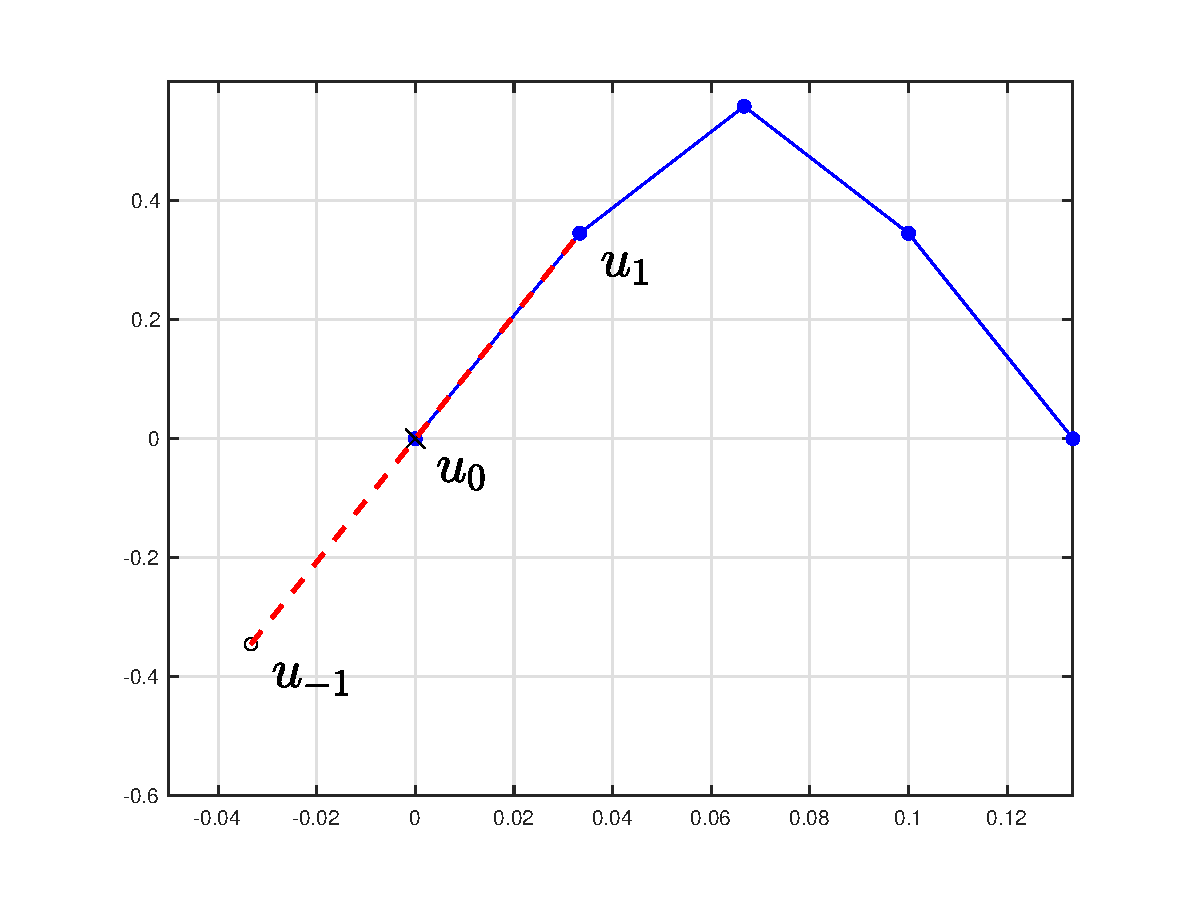
\includegraphics[width=0.6\columnwidth]{plot3.eps}}
% \caption{\label{fig:eta}{Boundary Condition. Curvature at $u_0$ needs to be 0.}}
% \end{figure}
\section{The Interpolated Boundary}
In this section, the location of a grid point $u_l$ along the string will be given by $x_l$. In the normal case, i.e., when the first grid point lays on the boundary ($x_0 = 0$), we can satisfy \eqref{eq:boundaryCondition} as follows:
\begin{equation}\label{eq:expandedBoundCond}
    \begin{aligned}
        &\delta_{xx}u_0 = 0\\
        &\frac{1}{h^2}(u_1 - 2u_0 + u_{-1}) = 0 \\[-13pt]
        \xLeftrightarrow{\mystrut\ u_0 = 0\ } \quad &u_{-1} = -u_1.
    \end{aligned}
\end{equation}
Applying this to an expanded version of Eq. \eqref{eq:1Dwave} is unnecessary, as we know that $u_0 = 0$ at all times, and therefore does not need to be updated. If $u_0$ doesn't lay on the boundary, however, we need to define and satisfy the boundary condition differently. Let's change the boundary condition to something more general to apply to a point $u_\text{B}$ which may or may not coincide with (or be equal to) $u_0$:
\begin{equation}\label{eq:generalBoundary}
        u_\text{B} = \delta_{xx}u_\text{B} = 0,
\end{equation}
where the location of the boundary along the string $x_\text{B} = 0$ at all times. Again, this condition states that the state as well as the curvature at the boundary needs to be 0. 

As $u_0$ is not necessarily $0$ (as it used to according to Eq. \eqref{eq:boundaryCondition}) we need to calculate it using the scheme in \eqref{eq:1Dwave}. We expand the scheme at $u_0$ and solve for $u_0^{n+1}$ as follows
\begin{equation}
    u_0^{n+1} = 2u_0^n - u_0^{n-1} + \lambda^2 (u_1^n - 2u_0^n+u_{-1}^n),
\end{equation}
where $\lambda = ck/h$. Now, we need a definition for virtual grid point $u_{-1}$, which we can obtain using the new boundary condition \eqref{eq:generalBoundary}.

In order to obtain a definition for the curvature at the boundary $\delta_{xx}u_\text{B}$, we need two points that are equally distant from the boundary. Starting from the virtual grid point $u_{-1}$ at the left side of the boundary, we can define some interpolated grid point $u_\text{I}$ with the same distance from the boundary as $u_{-1}$ (see Figure \ref{fig:dynamicBoundary} for a visualisation of this). 
\begin{figure}[h]
\centerline{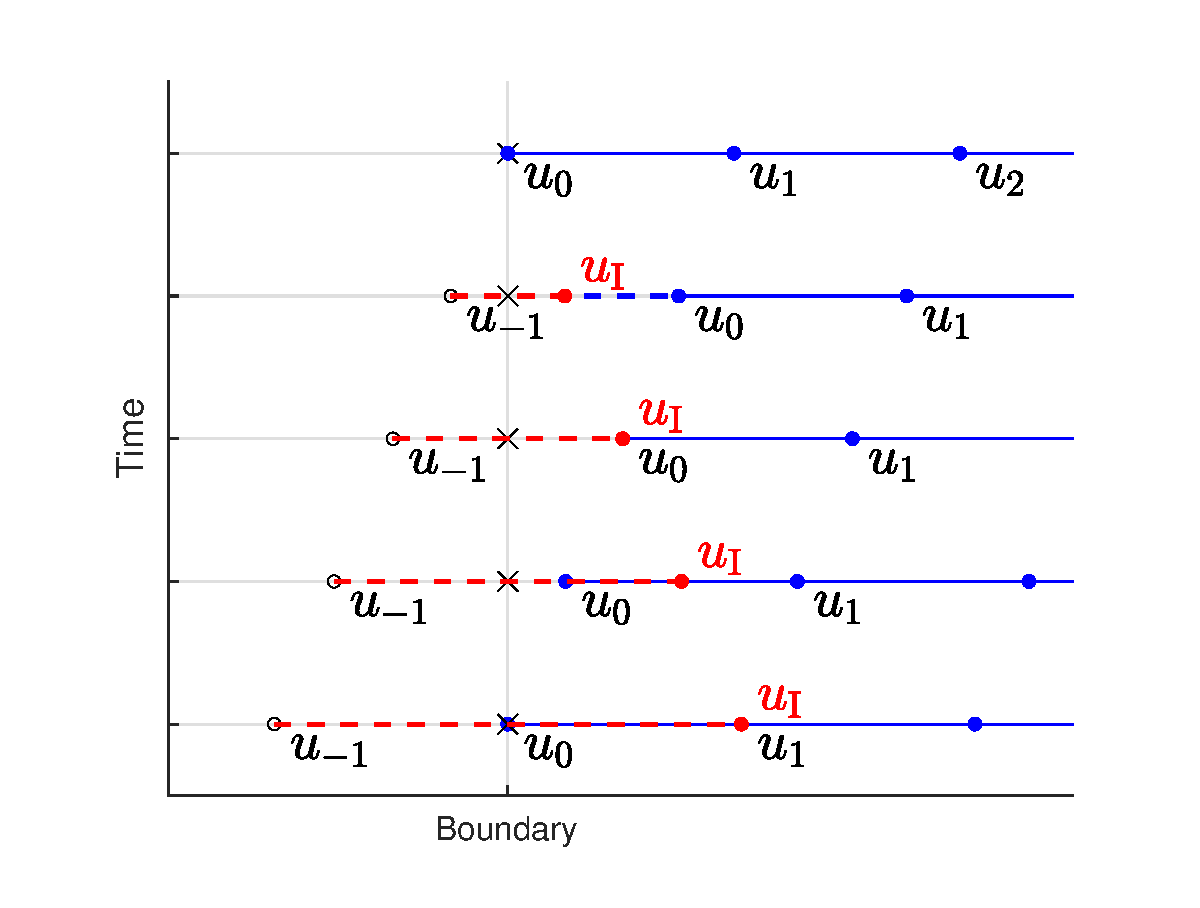
\includegraphics[width=0.6\columnwidth]{dynamicBoundaryDrawChange.eps}}
\caption{\label{fig:dynamicBoundary}{Boundary conditions at different values for $h$. Important to note is that the distance between $u_0$ and $u_{-1}$ always remains (the current) $h$. The distance between $u_{-1}$ and $u_\text{B}$ (and also $u_\text{I}$ and $u_\text{B}$) is defined as $h_\text{I}$. Then, from the location of $u_{-1}$, the location of $u_\text{I}$ (the interpolated point used to calculate the value of $u_{-1}$) is determined.}}
\end{figure}

This distance can be calculated using
\begin{equation}
    h_\text{I} = h - x_0,
\end{equation}
where $x_0$ is the location of $u_0$ along the string length. As $u_{-1}$ and $u_\text{I}$ have the same distance $h_\text{I}$ to the boundary and are at opposite sides, we can use these when expanding \eqref{eq:generalBoundary} and obtain a different definition for $u_{-1}$:
\begin{equation}
    \begin{aligned}
        &\delta_{xx}u_\text{B} = 0\\
        &\frac{1}{h_\text{I}^2} (u_\text{I} - 2u_\text{B} + u_{-1}) = 0\\[-13pt]
        \xLeftrightarrow{\mystrut\ u_\text{B} = 0\ } \quad & u_{-1} = - u_\text{I},
    \end{aligned}
\end{equation}
which is similar to condition \eqref{eq:expandedBoundCond}, but now using the interpolated state (or grid point) $u_\text{I}$. The last thing we need is a definition for this state which is currently done using linear interpolation. We do, however, need different definitions in the cases where $x_\text{I} > x_0$ (fourth instance from the top in Figure \ref{fig:dynamicBoundary}) and $x_\text{I} \leq x_0$ (second and third instance from the top in Figure \ref{fig:dynamicBoundary})
\begin{subequations}
    \begin{numcases}{}
        u_\text{I} = (1-\alpha) u_0 + \alpha u_1 \quad \text{where} \quad \alpha = \frac{h-2x_0}{h} &$ x_\text{I} > x_0$\label{eq:xiLarger}\\
        u_\text{I} = \underbrace{(1-\alpha) u_\text{B}}_{=0} + \alpha u_0 \quad \text{where} \quad \alpha = \frac{h_\text{I}}{x_0} &  $x_\text{I} \leq x_0$\label{eq:xiSmaller}
    \end{numcases}
\end{subequations}
% We can then use the distance of virtual grid point to $u_\text{B}$ to obtain a definition for it 

% Using $\lambda = ck/h$, expanding \eqref{eq:1Dwave} at the boundary and applying \eqref{eq:expandedBoundCond}:
% \begin{equation}
%     \begin{aligned}
%         u_0^{n+1} &= 2u_0^n - u_0^{n-1} + \lambda^2 (u_1^n-2u_0^n + u_{-1}^n)\\
%         \xLeftrightarrow{\text{Eq. \eqref{eq:expandedBoundCond}}}\quad u_0^{n+1} &= 2u_0^n - u_0^{n-1} + \lambda^2 (u_1^n-2u_0^n - u_1^n)\\
%         u_0^{n+1} &= 2u_0^n - u_0^{n-1} - 2\lambda^2 u_0^n
%     \end{aligned}
% \end{equation}
% we can see that the virtual grid point $u_{-1}$ essentially cancels out the effect that $u_1$ has on $u_0$.  
% satisfy the boundary condition: the curvature around the boundary needs to be $0$. 

\section{Energy}
We can get the energy of Eq. \eqref{eq:1Dwave} by first taking the inner product with respect to $\delta_{t\cdot}u$ like
\begin{equation}
    \delta_{t+}\mathfrak{h} = \rho A\langle \delta_{t\cdot}u, \delta_{tt}u\rangle_\mathcal{D} - T \langle \delta_{t\cdot}u,\delta_{xx}u\rangle_\mathcal{D} = 0,
\end{equation}
using integration by parts to get
\begin{equation}\label{eq:innerProd}
    \delta_{t+}\mathfrak{h} = \rho A\langle \delta_{t\cdot}u, \delta_{tt}u\rangle_\mathcal{D} + T \langle \delta_{t\cdot}\delta_{x+}u,\delta_{x+}u\rangle_{\underline{\mathcal{D}}} = \mathfrak{b},
\end{equation}
where boundary term
\begin{equation}
    \mathfrak{b} = T (\delta_{t\cdot}u_N)(\delta_{x+}u_N) - T(\delta_{t\cdot}u_0)(\underbrace{\delta_{x+}u_{-1}}_{\delta_{x-}u_0})\ .
\end{equation}
Expanding Eq. \eqref{eq:innerProd} yields,
\begin{equation}
    \delta_{t+}\mathfrak{h} = \rho A \sum_\mathcal{D}h(\delta_{t\cdot}u)(\delta_{tt}u) + T \sum_{\underline{\mathcal{D}}}h(\delta_{t\cdot}\delta_{x+}u)(\delta_{x+}u)
\end{equation}
Then, using the following identities  
\begin{subequations}
\begin{align}
    (\delta_{t\cdot}u)(\delta_{tt}u) &= \delta_{t+}\left(\frac{1}{2}(\delta_{t-}u)^2\right) \quad \text{and}\label{eq:identity1}\\
    (\delta_{t\cdot}u)u &= \delta_{t+}\left(\frac{1}{2}u e_{t-}u\right)\label{eq:identity2}
\end{align}
\end{subequations}
we can finally obtain the energy $\mathfrak{h}$:
\begin{gather}
        \mathfrak{h} = \mathfrak{t} + \mathfrak{v}\quad \text{where}\\
    \mathfrak{t} = \frac{\rho A}{2} \sum_{\mathcal{D}} h (\delta_{t-}u_l^n)^2 \quad \text{and} \quad \mathfrak{v} =  \frac{T}{2}\sum_{\underline{\mathcal{D}}}h (\delta_{x+}u_l^n)(\delta_{x+}u_l^{n-1})\nonumber
\end{gather}

In the case when $x_\text{I} \leq x_0$ (case \eqref{eq:xiSmaller}) we can find an energy definition for the left boundary:
\begin{equation}
    \begin{aligned}
        \delta_{t+}\mathfrak{h}_\text{l} &= T(\delta_{t\cdot}u_0)(\delta_{x-}u_0)\\
        &= \frac{T}{h}(\delta_{t\cdot}u_0)(u_0 - u_{-1})\\[-4pt]
        \xLeftrightarrow{\mystrut\ u_{-1} = -\alpha u_0\ } \quad & = \frac{T}{h}(\delta_{t\cdot}u_0)((1+\alpha)u_0)\\
        &= \frac{T(1+\alpha)}{h}(\delta_{t\cdot}u_0)u_0\\[-5pt]
        \xLeftrightarrow{\mystrut\ \text{Eq. \eqref{eq:identity2}}\ } \quad & = \frac{T(1+\alpha)}{h}\delta_{t+}\left(\frac{1}{2}u_0^nu_0^{n-1}\right)\\
        \mathfrak{h}_l &= \frac{T(1+\alpha)}{2h}u_0^nu_0^{n-1}
    \end{aligned}
\end{equation}
The next step will be to find the energy for case \eqref{eq:xiLarger} (if it exists....). Here follow the first steps:
\begin{equation}
    \begin{aligned}
        \delta_{t+}\mathfrak{h}_\text{l} &= T(\delta_{t\cdot}u_0)(\delta_{x-}u_0)\\
        &= \frac{T}{h}(\delta_{t\cdot}u_0)(u_0 - u_{-1})\\[-5pt]
        \xLeftrightarrow{\mystrut\ -u_{-1} = u_\text{I}\ \text{\&} \ \text{Eq. } \eqref{eq:xiLarger}\ } \quad & = \frac{T}{h}(\delta_{t\cdot}u_0)(u_0 + (1+\alpha) u_0 + \alpha u_1)\\
        &= \frac{T(2+\alpha)}{h}(\delta_{t\cdot}u_0)u_0 + \frac{T}{h}(\delta_{t\cdot}u_0)(\alpha u_1)\\[-5pt]
        \xLeftrightarrow{\mystrut\ \text{Eq. }\eqref{eq:identity2}\ } \quad &= \frac{T(2+\alpha)}{h}\delta_{t+}\left(\frac{1}{2}u_0^nu_0^{n-1}\right) + \underbrace{\frac{T}{h}(\delta_{t\cdot}u_0)(\alpha u_1)}_{\text{\SWcomment[The issue]}} 
    \end{aligned}
\end{equation}
\bibliographystyle{plain}
\bibliography{bibliography}

\appendix
\section{Note regarding issue when increasing $T$}\label{app:increasingT}
If we decrease $T$, the points smoothly enter the scheme without issues. However, in the opposite case when we increase $T$ (moving from top to bottom in Figure \ref{fig:dynamicGrid}), the string will already be moving at $u_0$ and continue moving due to its inertia (the $\rho A \delta_{tt}u$ term). In other words, even though we can satisfy the $\delta_{xx}u_0 = 0$ part of the boundary condition, $u_0=0$ is harder to satisfy. Something needs to be figured out for this..

\section{Alternative Approach: 1D-waves with connected free (Neumann) ends}
Another approach to changing the grid dynamically is to add / remove points in the center of the string rather than the boundaries (see Figure \ref{fig:twoFreeStrings}). I expect that doing this, rather than adding / removing points at the boundary, will allow for smoother changes when increasing $T$, i.e, when the amount of points decreases (see Appendix \ref{app:increasingT}). Consider a string, $u$ with $M_u = \text{ceil}(0.5/ck)$ (simply $M$ below for brevity) and $w$ with $M_w = \text{floor}(0.5/ck)$ points, i.e., half the number of points allowed by the stability condition $N$, plus one for overlap due to the combined $\text{ceil}$ $\text{floor}$ operations (will elaborate below). Then the following boundary conditions are imposed:
\begin{equation}\label{eq:halfStringBoundaryCond}
    \begin{aligned}
        u_0 = w_{M_w} &= 0,\quad \text{(Dirichlet)}\\
        \delta_{x\cdot}u_M = \delta_{x\cdot}w_0 &= 0\ \quad \text{(Neumann)}.
    \end{aligned}
\end{equation}

\begin{figure}[h]
\centerline{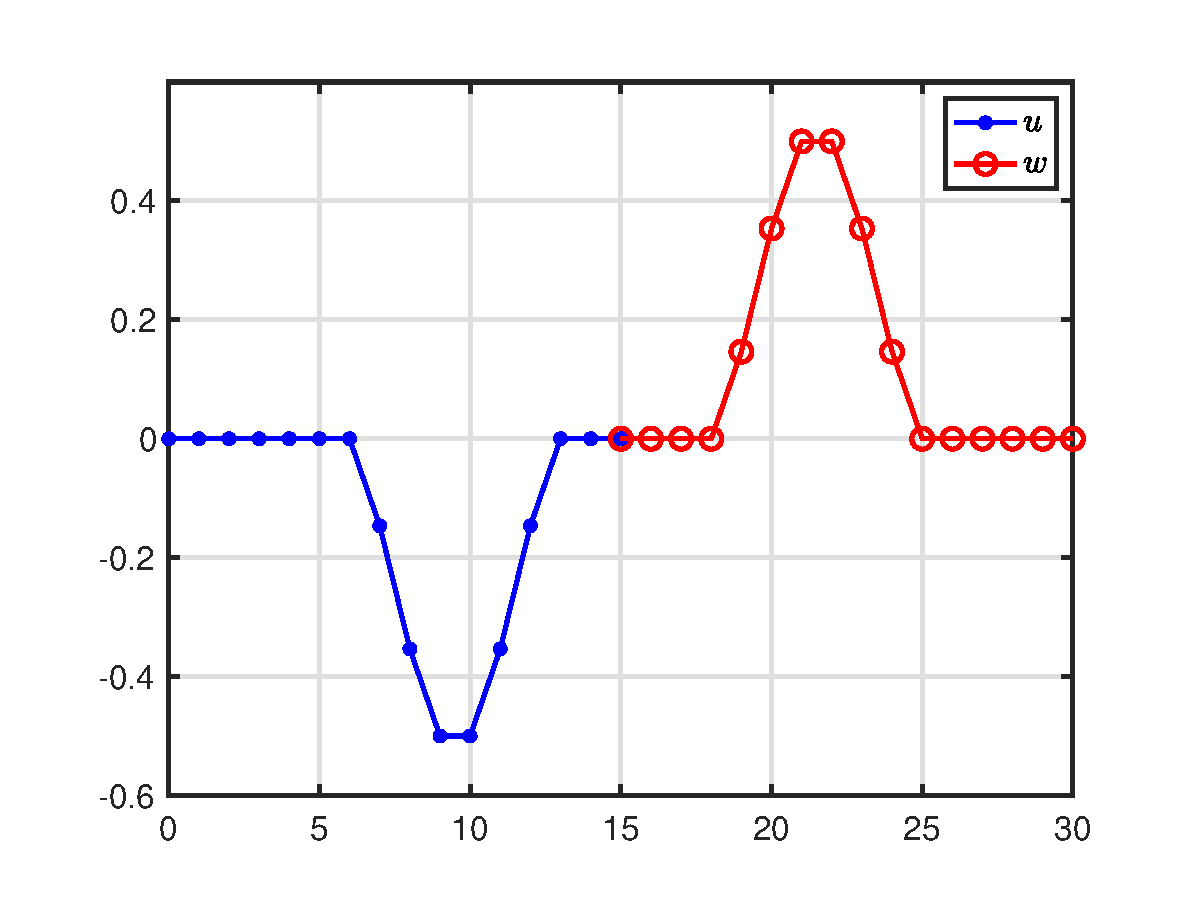
\includegraphics[width=0.6\columnwidth]{twoFreeStrings.eps} }
\caption{\label{fig:twoFreeStrings}{Two strings connected at one of their boundaries.}}
\end{figure}

\noindent Then we can connect $u_M$ and $w_0$ using a rigid connection, i.e.,
\begin{equation}\label{eq:rigid}
    u_M^n = w_0^n
\end{equation}
for all $n$. The system will now be
\begin{equation}
    \begin{cases}\label{eq:systemHalfStrings}
        \delta_{tt}u_l^n = c^2\delta_{xx}u_l^n + J(x_{u_M})F\\
        \delta_{tt}w_l^n = c^2\delta_{xx}w_l^n - J(x_{w_0})F
    \end{cases}
\end{equation}
where
\begin{equation}
    J(x_i) =
    \begin{cases}
        \frac{1}{h}, & l = l_i\\
        0,& \text{otherwise}
    \end{cases}
\end{equation}
If we expand the spatial derivative operators in \eqref{eq:systemHalfStrings} at $u_M$ and $w_0$ we get, recalling \eqref{eq:halfStringBoundaryCond}
\begin{equation}\label{eq:expandedSystem}
    \begin{cases}
        \delta_{tt}u_M^n = \frac{c^2}{h^2}(2u_{M-1}^n-2u_M^n) + \frac{1}{h}F\\
        \delta_{tt}w_0^n = \frac{c^2}{h^2}(2w_1^n-2w_0^n) - \frac{1}{h}F.
    \end{cases}
\end{equation}
Because \eqref{eq:rigid} is true we also know that $\delta_{tt}u_M^n = \delta_{tt}w_0^n$ for all $n$. We can then calculate $F$, by setting the equations in \eqref{eq:systemHalfStrings} equal to each other:

% \begin{equation}
% \begin{aligned}
%     c^2\delta_{xx}u_M^n + \frac{1}{h} F &= c^2\delta_{xx}w_0^n - \frac{1}{h} F\\
%     \frac{c^2}{h^2}(u_{M-1}^n-2u_M^n+u_{M+1}^n) + \frac{1}{h} F &= \frac{c^2}{h^2}(w_{-1}^n-2w_0^n+w_1^n) - \frac{1}{h} F
% \end{aligned}\nonumber
% \end{equation}

% \noindent Knowing through \eqref{eq:halfStringBoundaryCond} that $u_{M+1} = u_{M-1}$ and $w_{-1} = w_1$   yields
\begin{align}
     \frac{c^2}{h^2}(2u_{M-1}^n-2u_M^n) + \frac{1}{h} F&= 
     \frac{c^2}{h^2}(2w_1^n-2w_0^n) - \frac{1}{h} F\\
    \frac{2}{h}F &= \frac{c^2}{h^2}(2w_1^n - 2u_{M-1}^n)\nonumber\\
    F &= h \frac{c^2}{h^2}(w_1^n - u_{M-1}^n)
\end{align}
Filling this into \eqref{eq:expandedSystem} after expansion of the second-time derivative yields
\begin{subequations}\label{eq:resultOneConnectedPoint}
\begin{align}
    u^{n+1}_M &= 2u_M^n - u_M^{n-1} + \lambda^2(u_{M-1}^n-2u_M^n+\overbrace{w_1^n}^{u_{M+1}^n})\label{eq:resultOneConnectedPoint1}\\
    w^{n+1}_0 &= 2w_0^n - w_0^{n-1} + \lambda^2(\underbrace{u_{M-1}^n}_{w_{-1}^n}-2w_0^n+w_1^n)\label{eq:resultOneConnectedPoint2}
\end{align}
\end{subequations}
which, (again, recalling \eqref{eq:rigid}) are indeed equivalent expressions for the connected point. Here, $w_1$ in the first expression acts as virtual grid point $u_{M+1}^n$ and $u_{M-1}^n$ as virtual grid point $w_{-1}^n$. So essentially, to connect the two strings we add a state of one string to the update of the other.

\subsection{Changing the grid}
The previous is an exact solution to the problem when the stability condition is satisfied with equality, i.e, when $1/ck$ is an integer. If we then want to change the grid spacing according to $h=ck$ we leave the locations of the outer boundaries ($u_0$ and $w_{M_w}$) fixed and move the rest of the points towards their respective outer boundary (see Figure \ref{fig:interpolated}). 

We now continue with the idea of adding a state of one string in the update of the other. When the stability condition is not satisfied with equality -- and thus the points of the strings don't overlap -- we use linear interpolator $I_1$. This results in,
\begin{align}
    u_{M+1}^n &= I_1(x_{u_{M+1}})w_l^n = (1-\alpha)w_1^n + \alpha w_0^n\\
    w_{-1}^n &= I_1(x_{w_{-1}})u_l^n = (1-\alpha)u_{M-1}^n + \alpha u_M^n
\end{align}
where
\begin{equation}
    \alpha = \frac{x_{w_0} - x_{u_M}}{h},
\end{equation}
and grid-point locations $x_{u_{M+1}}$ and $w_{-1}$. Note that when $h$ changes the connected points start to move away from each other.
\begin{figure}[h]
    \centering
    \subfloat[When $h$ changes.]{\label{fig:interpolatedFull}{ 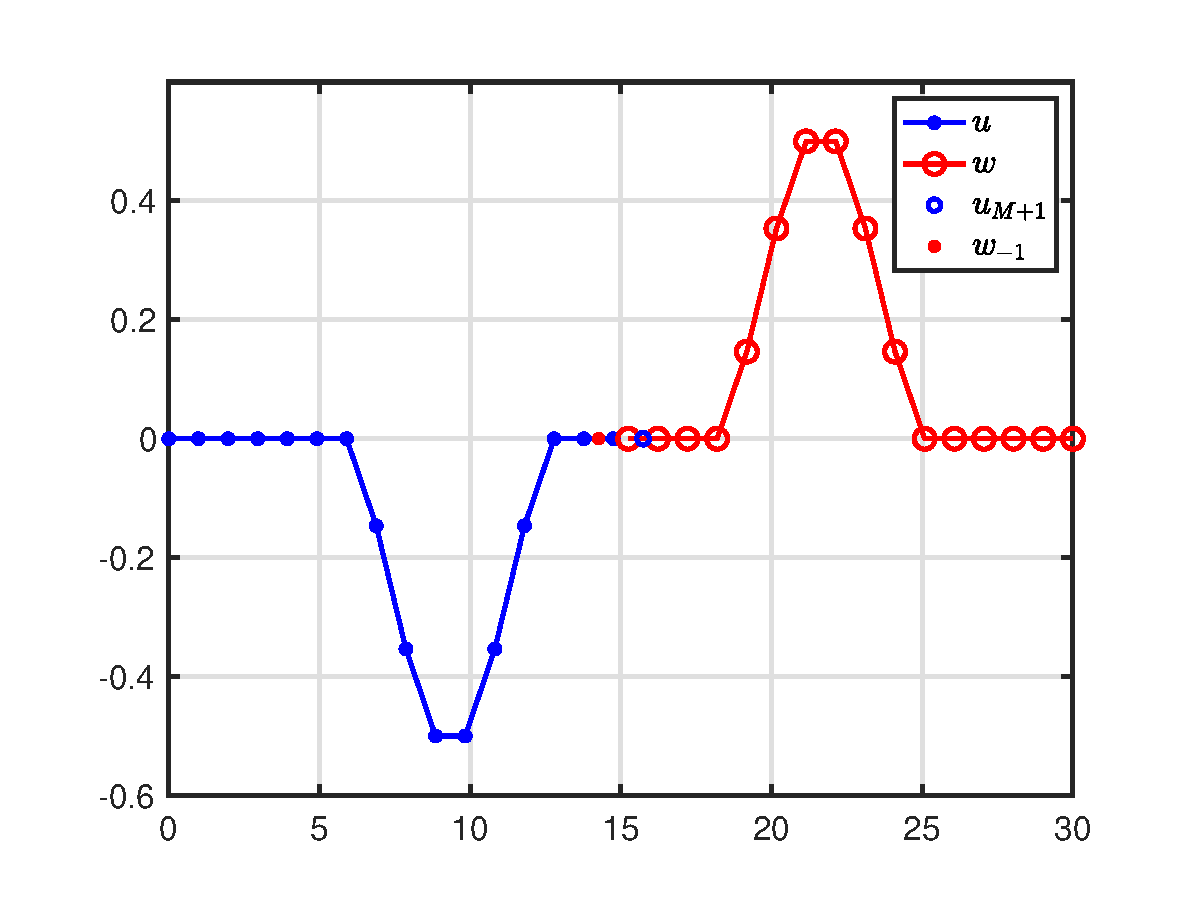
\includegraphics[width=0.5\textwidth]{twoFreeStringsInterpolatedFull.eps}}}
    \subfloat[Zoomed]{\label{fig:interpolatedZoom}{ 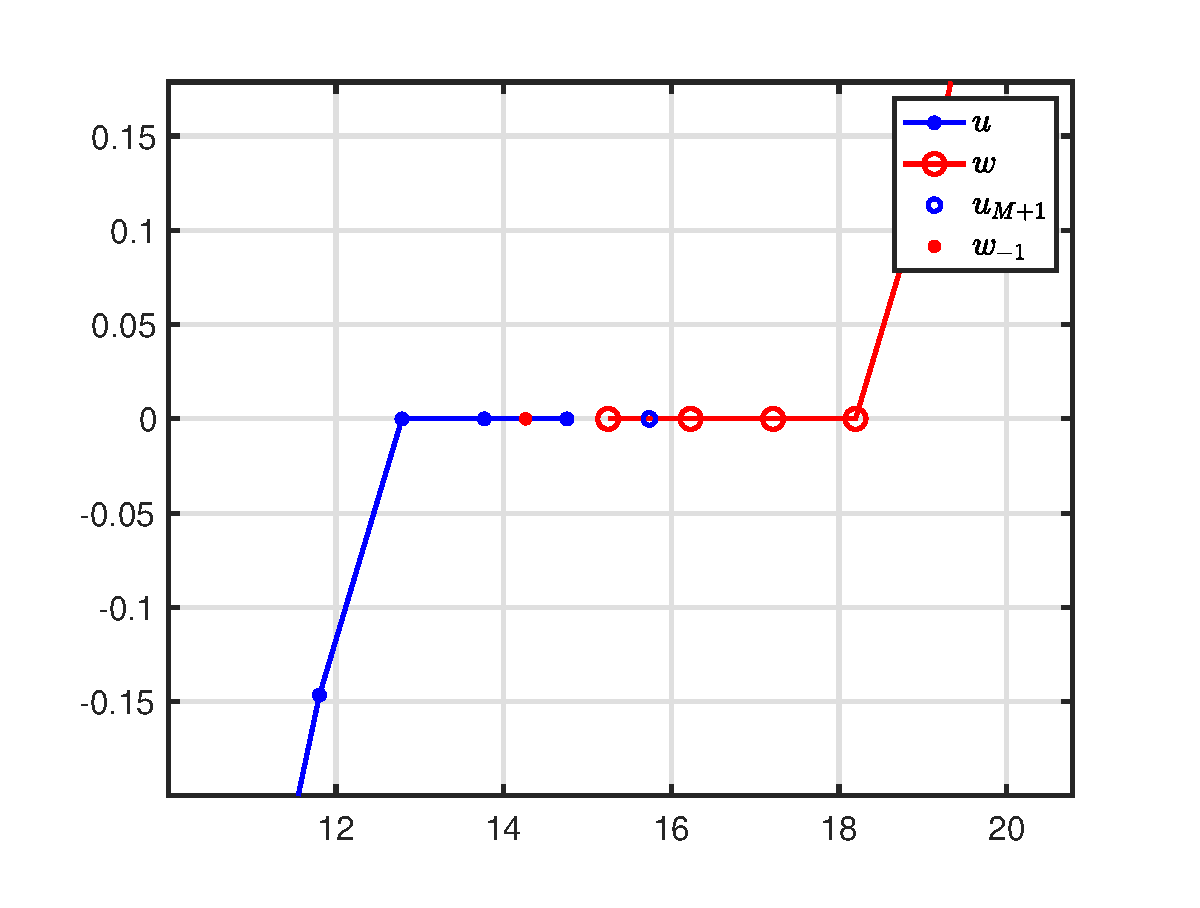
\includegraphics[width=0.5\textwidth]{twoFreeStringsInterpolated.eps}}}
    \caption{}\label{fig:interpolated}
\end{figure}
%
Then, when the boundary points surpass with the virtual points (i.e. $x_{u_M} \leq x_{w_{-1}}$ and $x_{u_{M+1}} \leq x_{w_0}$) we alternate between adding / removing a point to the right side of $u$ and the left side of $w$.
\begin{equation}\label{eq:addingRemovingPoints}
    \begin{cases}
        \begin{cases}\u^n = [\u^n, \mathcal{I}(x_{u_{M+1}})\mathbf{v}^n]^T & \text{if $N^n$ is odd}\\
        \mathbf{w}^n = [\mathcal{I}(x_{w_{-1}})\mathbf{v}_\star^n, \mathbf{w}^n]^T & \text{if $N^n$ is even}
        \end{cases} & \text{if } N^n > N^{n-1} \text{ (adding a point)}\\
        \\
        \begin{cases}
        \u^n = [u_0^n, u_1^n ..., u_{M-1}^n]^T & \text{if $N^n$ is even} \\
         \mathbf{w}^n = [w_1^n, w_2^n ..., w_{M_w}^n]^T & \text{if $N^n$ is odd} 
        \end{cases} &\text{if } N^n < N^{n-1} \text{ (removing a point)}
        % u^{n-1} = [u^{n-1}, I(x_{u_{M+1}})w^{n-1}];
    \end{cases}
\end{equation}
where
\begin{align}
    \mathbf{v}^n &= [u_{M-1}^n, u_M^n, w_0^n, w_1^n]^T \quad \text{and}\\
    \mathbf{v}_\star^n &= [w_1^n, w_0^n, u_M^n, u_{M-1}^n]^T
\end{align}
Figure \ref{fig:addingPoint} shows a point being added to the grid
\begin{figure}[h]
\centerline{\includegraphics[width=0.6\columnwidth]{addingPoint.eps} }
\caption{\label{fig:addingPoint}{Point added to the grid according to \eqref{eq:addingRemovingPoints} (at the boundary though..)}}   
\end{figure}

The interpolator used is (cubic Lagrange)
\begin{equation}\label{eq:customInterp}
    \mathcal{I} = \begin{bmatrix} -\frac{\alpha(\alpha+1)}{(\alpha+2)(\alpha+3)} &\frac{2\alpha}{\alpha+2} &\frac{2}{\alpha+2} 
    &-\frac{2\alpha}{(\alpha+3)(\alpha+2)}
    \end{bmatrix},
\end{equation}
with
\begin{equation}
    \alpha = \frac{x_{w_0} - (x_{u_M} + h)}{h}\ .
\end{equation}
See section \ref{sec:lagrangeDeriv} for a derivation of Eq. \eqref{eq:customInterp}.

Even though subjective listening confirmed that the sound is smooth when adding / removing points using linear interpolation, the expected fundamental frequency ($f_0 \approx c/2$) was slightly too high when interpolation needed to happen. Instead of a linear, the cubic interpolator $I_3$ can be used according to 
% \begin{equation}\label{eq:connectionInterpol}
%     \begin{aligned}
%         u_{M+1}^n = I_3(x_{u_{M+1}})w_l^n &= \frac{\alpha(\alpha - 1)(\alpha - 2)}{-6} w_2^n + \frac{(\alpha - 1)(\alpha + 1)(\alpha - 2)}{2}w_1^n \\
%         &+ \frac{\alpha(\alpha + 1)(\alpha - 2)}{-2}w_0^n + \frac{\alpha(\alpha + 1)(\alpha - 1)}{6} w_{-1}^n\\
%         w_{-1}^n = I_3(x_{w_{-1}})u_l^n &= \frac{\alpha(\alpha - 1)(\alpha - 2)}{-6} u_{M-2}^n + \frac{(\alpha - 1)(\alpha + 1)(\alpha - 2)}{2}u_{M-1}^n \\
%         &+ \frac{\alpha(\alpha + 1)(\alpha - 2)}{-2}u_M^n + \frac{\alpha(\alpha + 1)(\alpha - 1)}{6} u_{M+1}^n.
%     \end{aligned}
% \end{equation}

\begin{equation}\label{eq:connectionInterpol}
    \begin{aligned}
        u_{M+1}^n &= I_3(x_{u_{M+1}})w_l^n &&= \alpha_\text{I}w_2^n + \beta_\text{I}w_1^n + \gamma_\text{I}w_0^n + \delta_\text{I} w_{-1}^n\\
        w_{-1}^n &= I_3(x_{w_{-1}})u_l^n &&=\alpha_\text{I} u_{M-2}^n + \beta_\text{I}u_{M-1}^n+ \gamma_\text{I}u_M^n + \delta_\text{I} u_{M+1}^n.
    \end{aligned}
\end{equation}
where
\begin{gather*}
    \alpha_\text{I} = \frac{\alpha(\alpha - 1)(\alpha - 2)}{-6}, \quad \beta_\text{I} = \frac{(\alpha - 1)(\alpha + 1)(\alpha - 2)}{2},\\
    \gamma_\text{I} = \frac{\alpha(\alpha + 1)(\alpha - 2)}{-2}, \quad \text{and} \quad\delta_\text{I} = \frac{\alpha(\alpha + 1)(\alpha - 1)}{6}\,.
\end{gather*}
We can solve for $u_{M+1}^n$ and $w_{-1}^n$ by treating \eqref{eq:connectionInterpol} as a linear system of equations
\begin{equation}\label{eq:matSolution}
    \begin{bmatrix}
    u_{M+1}^n \\
    w_{-1}^n
    \end{bmatrix}
    =
    \mathbf{A}^{-1}
    \mathbf{v},
\end{equation}
where
% \begin{equation}\nonumber
%     \mathbf{A} = \begin{bmatrix}
%          1 & -\frac{\alpha(\alpha + 1)(\alpha - 1)}{6} \\
%          -\frac{\alpha(\alpha + 1)(\alpha - 1)}{6} & 1
%     \end{bmatrix},
% \end{equation}
% and
% \begin{equation}\nonumber
%     \mathbf{v} = \begin{bmatrix}
%     \frac{\alpha(\alpha - 1)(\alpha - 2)}{-6} w_2^n+ \frac{(\alpha - 1)(\alpha + 1)(\alpha - 2)}{2}w_1^n + \frac{\alpha(\alpha + 1)(\alpha - 2)}{-2}w_0^n \\
%     \frac{\alpha(\alpha - 1)(\alpha - 2)}{-6} u_{M-2}^n + \frac{(\alpha - 1)(\alpha + 1)(\alpha - 2)}{2}u_{M-1}^n + \frac{\alpha(\alpha + 1)(\alpha - 2)}{-2}u_{M}^n
%     \end{bmatrix}.
% \end{equation}

\begin{equation}\label{eq:Av}
    \mathbf{A}
    =
     \begin{bmatrix}
         1 & -\delta_\text{I} \\
         -\delta_\text{I} & 1
    \end{bmatrix} \quad \text{and} \quad \mathbf{v} = \begin{bmatrix}
    \alpha_\text{I} w_2^n+ \beta_\text{I}w_1^n + \gamma_\text{I}w_0^n \\
    \alpha_\text{I} u_{M-2}^n + \beta_\text{I}u_{M-1}^n + \gamma_\text{I} u_{M}^n
    \end{bmatrix}.
\end{equation}

Using cubic interpolation gives us the expected fundamental frequency for any wave speed. This can be proven using modal analysis, described in \ref{sec:modal}.

\subsubsection{Derivation of the LaGrange interpolator}\label{sec:lagrangeDeriv}
This subsection shows a derivation of how to get to Eq. \eqref{eq:customInterp}. We use Lagrange interpolation defined as
\begin{equation}\label{eq:lagrangeForm}
    \mathcal{I}_i = \prod_{k = 0, k\neq i}^m \frac{x-x_k}{x_i-x_k}.
\end{equation}
We then need the locations of the points we are using to interpolate. If we let (normalised by $h$ as all of the terms contain it)
\begin{equation}
    \begin{aligned}
     x_0 &= x_{u_{M-1}} = 0, \quad \text{then}\\
     x_1 &= x_{u_M} = 1, \\
     x_2& = x_{w_0} = 2 + \alpha , \quad \text{and}\\
     x_3 &= x_{w_1} = 3 + \alpha .
    \end{aligned}
\end{equation}
The $x$ that we're solving for is 
\begin{equation}
    x = x_{u_M+1} = 2\ .
\end{equation}
As all of these contain a multiplication with $h$, these can be divided out. The interpolator can then be built as follows:

\begin{align}
    \mathcal{I}_0 &= \left(\frac{2-1}{0-1}\right)\left(\frac{2-(\alpha+2)}{0-(\alpha+2)}\right)\left(\frac{2-(\alpha+3)}{0-(\alpha+3)}\right)= \left(-1\right)\left(\frac{-\alpha}{-(\alpha+2)}\right)\left(\frac{-(\alpha+1)}{-(\alpha+3)}\right)\nonumber\\
    &= -\frac{\alpha(\alpha+1)}{(\alpha+2)(\alpha+3)}\\
    \mathcal{I}_1 &= \left(\frac{2-0}{1-0}\right)\left(\frac{2-(\alpha+2)}{1-(\alpha+2)}\right)\left(\frac{2-(\alpha+3)}{1-(\alpha+3)}\right) = \left(2\right)\left(\frac{-\alpha}{-(\alpha+1)}\right)\left(\frac{-(\alpha+1)}{-(\alpha+2)}\right)\\
    &= \frac{2\alpha}{\alpha+2}\\
    \mathcal{I}_2 &= \left(\frac{2-0}{(\alpha+2)-0}\right)\left(\frac{2-1}{(\alpha+2)-1}\right)\left(\frac{2-(\alpha+3)}{(\alpha+2)-(\alpha+3)}\right) = \left(\frac{2}{\alpha+2}\right) \left(\frac{1}{\alpha+1}\right)\left(\frac{-(\alpha+1)}{-1}\right)\\
    &= \frac{2}{\alpha+2}\\
    \mathcal{I}_3 &= \left(\frac{2-0}{(\alpha+3)-0}\right)\left(\frac{2-1}{(\alpha+3)-1}\right)\left(\frac{2-(\alpha+2)}{(\alpha+3)-(\alpha+2)}\right) = \left(\frac{2}{\alpha+3}\right)\left(\frac{1}{\alpha+2}\right)\left(\frac{-\alpha}{1}\right) \\
    &= -\frac{2\alpha}{(\alpha+3)(\alpha+2)}
\end{align}

\subsection{Sinc interpolation}
An even better result is obtained using \textit{sinc interpolation}. 

\subsubsection{Introduction}
One can retrieve a continuous-time signal $y(t)$ from a discrete time-series $y[n]$ using 
\begin{equation}\label{eq:generalSincIP}
    y(t) = \sum_{n = -\infty}^{\infty} y[n] \cdot \text{sinc}\left(\frac{t - nT}{T}\right).
\end{equation}
where the normalised sinc function is defined as
\begin{equation}\label{eq:sinc}
    \text{sinc}(x) = \begin{cases}
        \frac{\sin(\pi x)}{\pi x} & x\neq 0\\
        1 & x = 0.
    \end{cases}
\end{equation}
Also see Figure \ref{fig:sinc}.
\begin{figure}[h]
\centerline{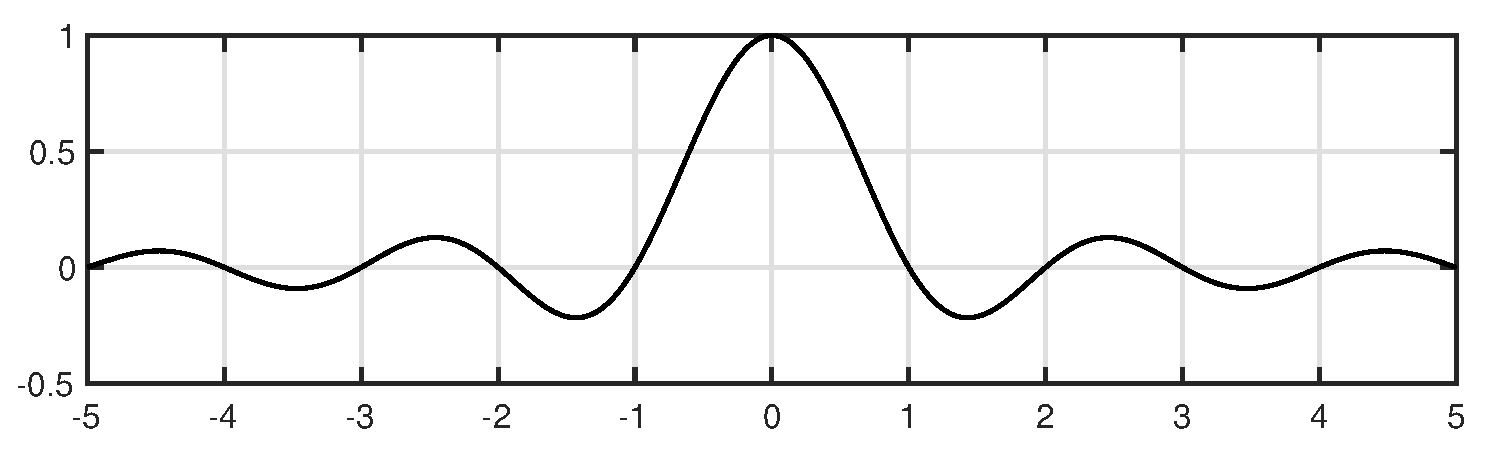
\includegraphics[width=0.6\columnwidth]{sincFig.eps} }
\caption{\label{fig:sinc}{Sinc function in Eq. \eqref{eq:sinc} truncated at $x = -5$ and $x = 5$.}}
\end{figure}


Naturally, \eqref{eq:generalSincIP} can not be implemented ``as is", due to the infinite sum. The continuous-time signal $y$ can, however, be quite well approximated even with a truncated version of Eq. \eqref{eq:generalSincIP}.

Going from DSP back to FDTD methods, \eqref{eq:generalSincIP} can be rewritten in terms we already know and applied to grid function $u$ in space (rather than time)
\begin{equation}\label{eq:FDSSinc}
    u(x^\star) = \sum_{l = \mathcal{D}_\text{i}} u_l \cdot \text{sinc}\left(\frac{x^\star - lh}{h}\right).
\end{equation}
where $\mathcal{D}_\text{i}$ is the range for interpolation. Ideally, one uses the entire known domain of 

\begin{figure}[h]
\centerline{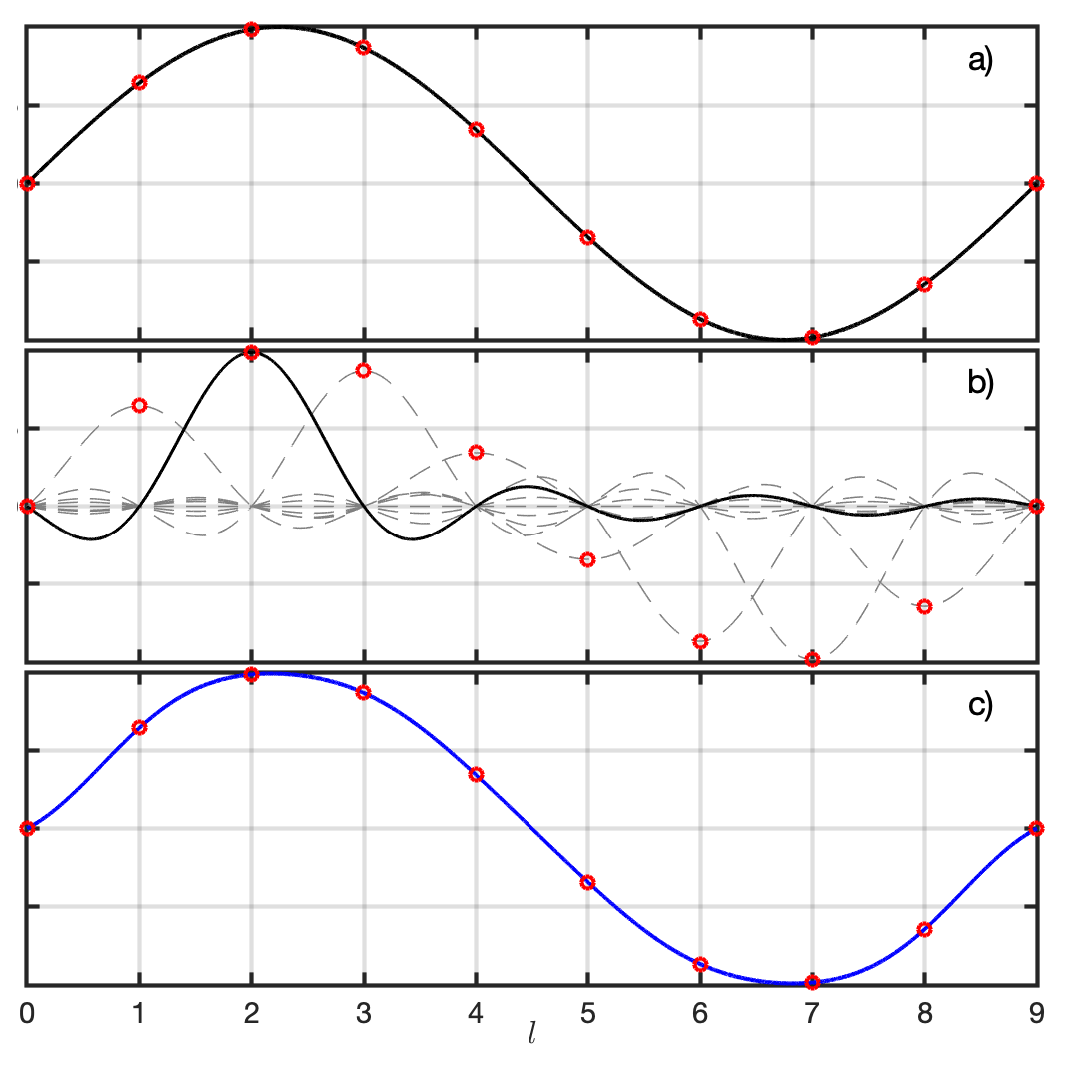
\includegraphics[width=0.6\columnwidth]{sincExplanation.eps} }
\caption{\label{fig:sincExp}{Explanation of sinc interpolation in Eq. \eqref{eq:FDSSinc}. a) The ``true" state of the system is sinusoidal and is sampled at $l \in [0, 9]$ marked in red. b) Sinc functions with their centers at the sampled points scaled by the value of $u_l$ are drawn in grey with the one centered at $l = 2$ highlighted in black. Notice that exactly at a sample point $l$, all functions are 0 except for the one centered at $l$. c) The interpolated system is retrieved by adding all the functions in b) and plotted in blue. The interpolated state is almost identical to the true state shown in a).}}
\end{figure}



\subsection{Modal Analysis}\label{sec:modal}
In order to analyse the behaviour of the interpolator, one can perform a modal analysis. It is possible to write the complete system in matrix form as
\begin{equation}
    \U^{n+1} = \mathbf{B}\U^n - \U^{n-1}
\end{equation}
where \begin{equation}\label{eq:uVecDef}
\U^n = \begin{bmatrix}
u^n_1, \hdots, u^n_M, w_0^n, \hdots, w_{M_w-1}  ^n
\end{bmatrix}^T,
\end{equation}
(so $\U^n$ and $\mathbf{w}^n$ concatenated excluding the outer boundaries).  The modal frequencies (eigenfrequencies) of the system can then be calculated using the following formula \cite[p. 174]{Bilbao2009}

\begin{equation}\label{eq:modalAnalysis}
    f_p = \frac{1}{2\pi k}\cos^{-1}\left(\frac{1}{2}\text{eig}_p(\mathbf{B})\right).
\end{equation}
If $\alpha = 0$, i.e., $x_{u_M} = x_{w_0}$ $\mathbf{B}$ looks like
\begin{equation}\label{eq:alphaIs0Full}
    \mathbf{B} = 2\mathbf{I} + \lambda^2 \begin{bmatrix}[cccccc|cccccc]
        &-2 & 1 & & & & & & & & & \\
        &1 & -2 & 1 & & & & & & & & \\
        &  & \ddots  &\ddots & \ddots & & & & 0 & & & \\
       & & & 1 & -2 & 1 &  & & & & & \\
       && & & 1 & -2 & 0 & 1 & & & & \\ \cline{2-11}
      & & & & 1 & 0 &-2 & 1 & & & & \\
         & & & & & &1 & -2 & 1 & & & \\
         & & & 0 & & &  & \ddots  &\ddots & \ddots & & \\
        & & & & & & & & 1 & -2 & 1 & \\
        & & & & & & & & & 1 & -2 & 
    \end{bmatrix}
\end{equation}
As $\lambda = 1$ at all times we can write \eqref{eq:alphaIs0Full} as 
\begin{equation}\label{eq:alphaIs0}
    \mathbf{B} = \begin{bmatrix}[cccccc|cccccc]
        &0 & 1 & & & & & & & & & \\
        &1 & 0 & 1 & & & & & & & & \\
        &  & \ddots  &\ddots & \ddots & & & & 0 & & & \\
       & & & 1 & 0 & 1 &  & & & & & \\
       && & & 1 & 0 & 0 & 1 & & & & \\ \cline{2-11}
      & & & & 1 & 0 &0 & 1 & & & & \\
         & & & & & &1 & 0 & 1 & & & \\
         & & & 0 & & &  & \ddots  &\ddots & \ddots & & \\
        & & & & & & & & 1 & 0 & 1 & \\
        & & & & & & & & & 1 & 0 & 
    \end{bmatrix}
\end{equation}
The $1$'s in the top-right and bottom-left quadrant show the interaction between $\U$ and $\mathbf{w}$ as shown in \eqref{eq:resultOneConnectedPoint}. In other words, $u_M^n$ is calculated using $w_1^n$ and $w_0^n$ using $u_{M-1}^n$. The following subsections show the experiments done with the three different types of interpolation mentioned in the previous section, i.e., linear, cubic and sinc interpolation.

\subsubsection{Linear interpolation}
We can change $\mathbf{B}$ to include linear interpolation using (focusing only on the middle of the matrix)
% \begin{equation}
%     \mathbf{B}_1 = 2\mathbf{I} + \lambda^2 \begin{bmatrix}[cccccc|cccccc]
%         &-2 & 1 & & & & & & & & & \\
%         &1 & -2 & 1 & & & & & & & & \\
%         &  & \ddots  &\ddots & \ddots & & & & 0 & & & \\
%       & & & 1 & -2 & 1 &  & & & & & \\
%       && & & 1 & -2 & \alpha & (1-\alpha) & & & & \\ \cline{2-11}
%       & & & & (1-\alpha) & \alpha &-2 & 1 & & & & \\
%          & & & & & &1 & -2 & 1 & & & \\
%          & & & 0 & & &  & \ddots  &\ddots & \ddots & & \\
%         & & & & & & & & 1 & -2 & 1 & \\
%         & & & & & & & & & 1 & -2 & 
%     \end{bmatrix}
% \end{equation}

\begin{equation}
    \mathbf{B}_1 = \begin{bmatrix}[cccc|cccc]
     & \ddots  &\ddots & & & & 0 & \\
       & 1 & 0 & 1 & & & & \\
      & & 1 & 0 & \alpha & (1-\alpha) & \\ \cline{2-7}
      & & (1-\alpha) & \alpha &0 & 1 & & \\
         & & & &1 & 0 & 1  \\
         & 0 & &  &  &\ddots & \ddots &
    \end{bmatrix}
\end{equation}

\begin{figure}[h]
    \centering
    \subfloat[Modal analysis for linear interpolation.]{\label{fig:linearModesAddInCenter}{ 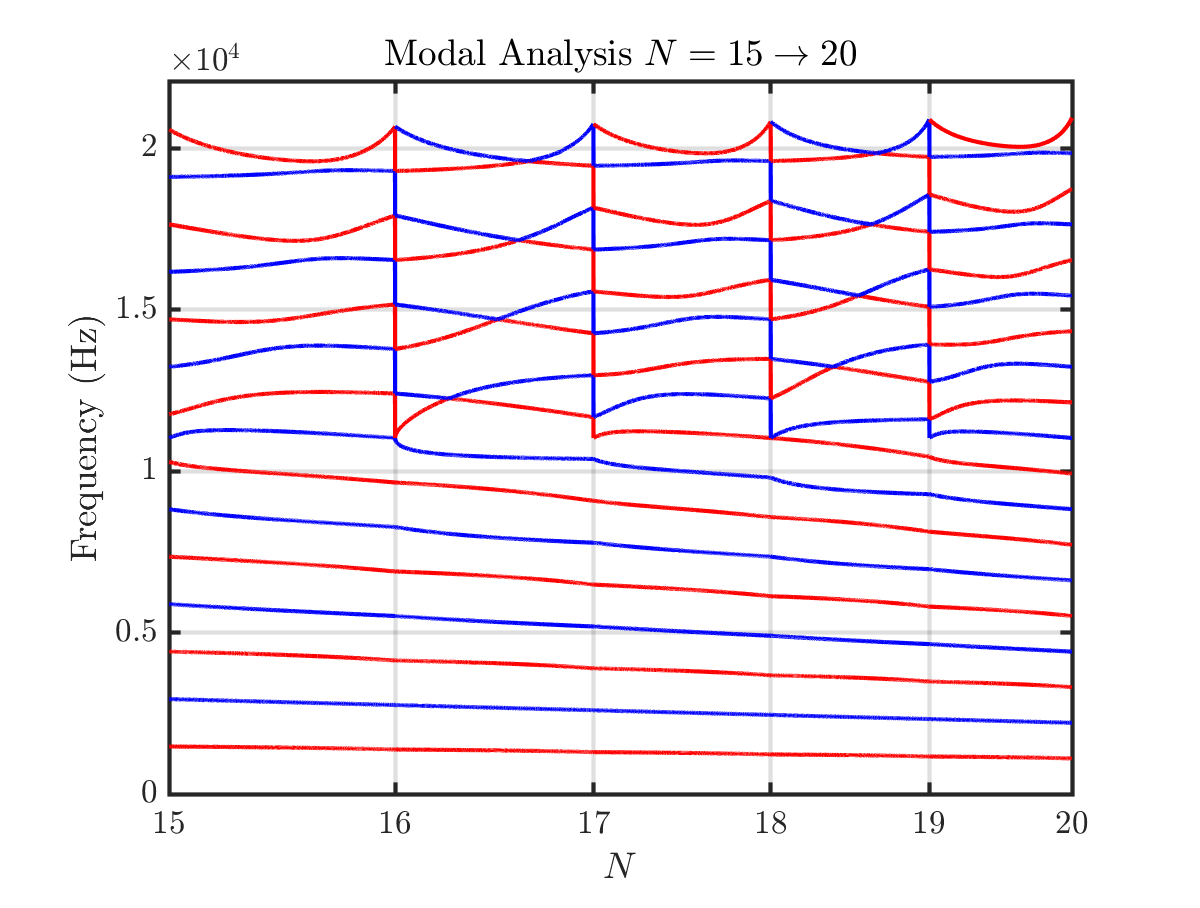
\includegraphics[width=0.45\textwidth]{modalAnalysisFigs/linearMid.eps}}}
    \hspace{0.05\textwidth}
    \subfloat[Spectrogram of system wave excited with raised cosine when $N = 15$.]{\label{fig:specLinAddCenter}{ 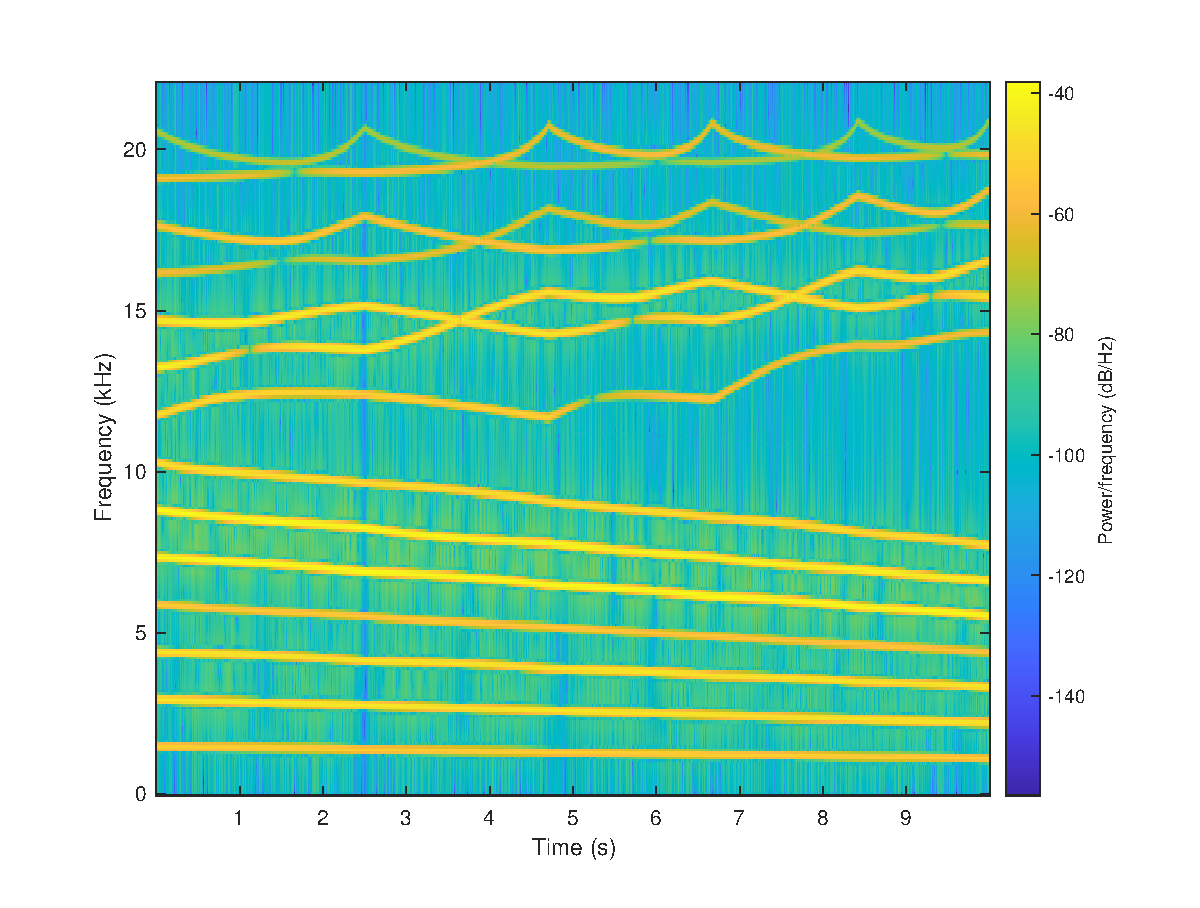
\includegraphics[width=0.45\textwidth]{modalAnalysisFigs/specLinearMid.eps}}}
    \caption{1D wave going linearly from $c = 2940$ m/s ($N=15$) to $c =2205$ m/s ($N=20$). Points are added in the middle.}\label{fig:linAddInCenter}
\end{figure}
\subsubsection{Quadratic Interpolation}
One could increase the number of points to take into account in the interpolation. Here we use $u_{M}$, $w_0$ and $w_1$ to calculate $u_{M+1}$. The matrix then becomes
\begin{equation}\label{eq:quadMat}
    \mathbf{B}_2 = \begin{bmatrix}[cccc|cccc]
     & \ddots  &\ddots & & & & 0 & \\
       & 1 & 0 & 1 & & & & \\
      & & 1 & \frac{\alpha - 1}{\alpha + 1} & 1 & -\frac{\alpha - 1}{\alpha + 1} & \\ \cline{2-7}
      & & -\frac{\alpha - 1}{\alpha + 1} & 1 & \frac{\alpha - 1}{\alpha + 1} & 1 & & \\
         & & & &1 & 0 & 1  \\
         & 0 & &  &  &\ddots & \ddots &
    \end{bmatrix}
\end{equation}
\begin{figure}[h]
    \centering
    \subfloat[Modal analysis for linear interpolation.]{\label{fig:quadModesAddInCenter}{ 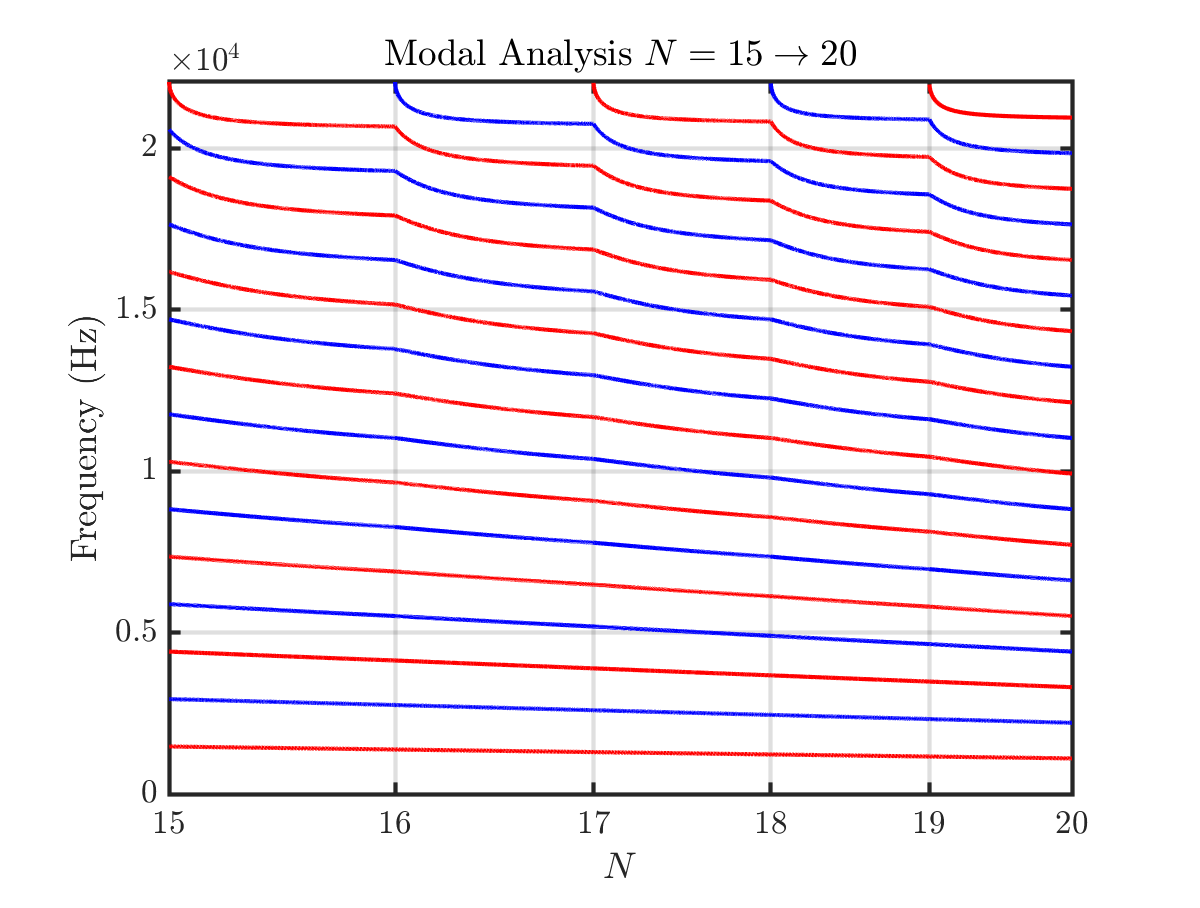
\includegraphics[width=0.45\textwidth]{modalAnalysisFigs/quadraticMid.eps}}}
    \hspace{0.05\textwidth}
    \subfloat[Spectrogram of system wave excited with raised cosine when $N = 15$.]{\label{fig:specQuadAddCenter}{ 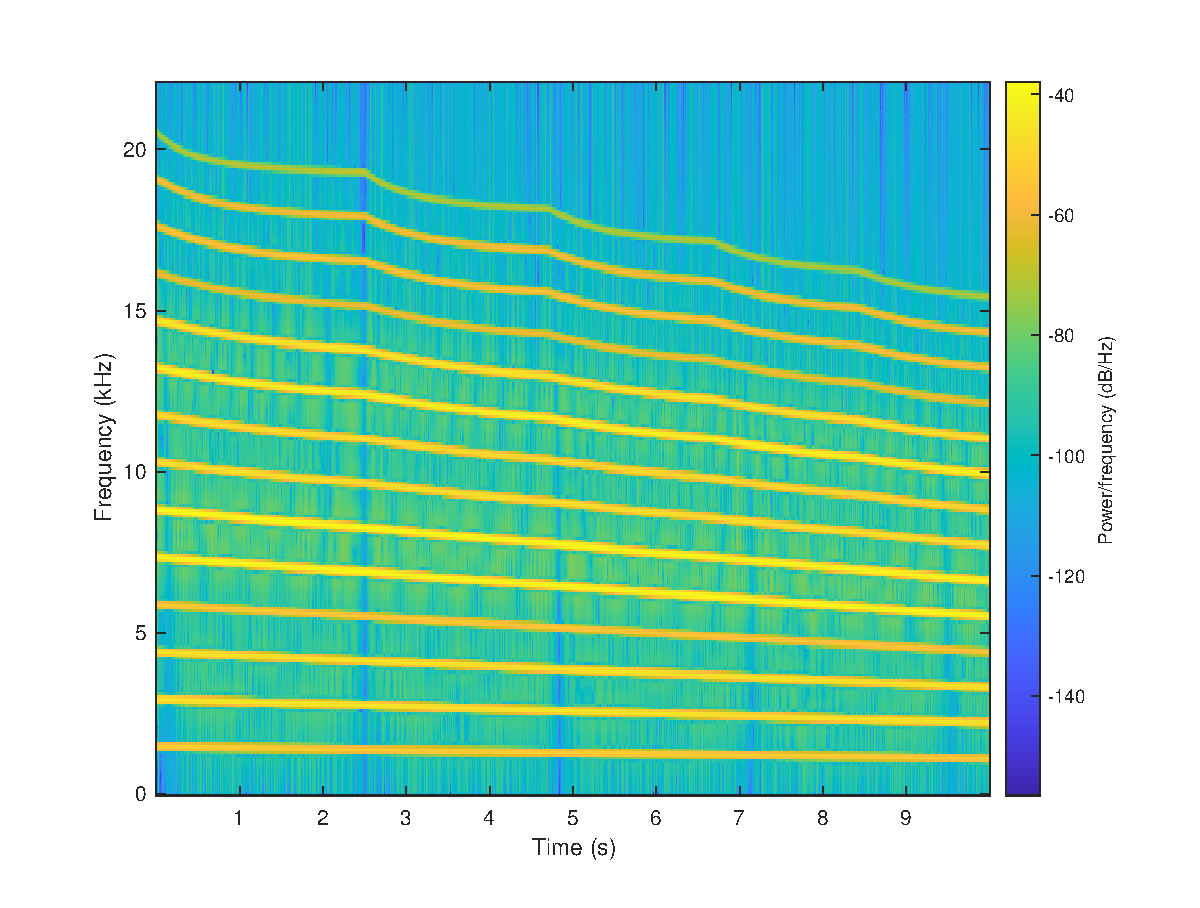
\includegraphics[width=0.45\textwidth]{modalAnalysisFigs/specQuadraticMid.eps}}}
    \caption{1D wave going linearly from $c = 2940$ m/s ($N=15$) to $c =2205$ m/s ($N=20$). Points are added in the middle.}\label{fig:linAddInCenter}
\end{figure}
\subsubsection{Cubic Interpolation}
\subsubsection*{Equally spaced grid points}
Cubic interpolation (using equally spaced points) is slightly trickier but still possible. Renaming $\mathbf{A}^{-1}$ from Eq. \eqref{eq:Av} to $\mathbf{A}^\text{i}$ and writing out \eqref{eq:matSolution} yields
\begin{align}
    u_{M+1}^n = \mathbf{A}^\text{i}_{1, 1}\begin{bmatrix}
   \gamma_\text{I} & \beta_\text{I} & \alpha_\text{I}
    \end{bmatrix} \begin{bmatrix}
   w_0^n & w_1^n &w_2^n
    \end{bmatrix}^T + \mathbf{A}^\text{i}_{1, 2}\begin{bmatrix}
   \alpha_\text{I} & \beta_\text{I} & \gamma_\text{I}
    \end{bmatrix} \begin{bmatrix}
   u_{M-2}^n & u_{M-1}^n &u_M^n
    \end{bmatrix}^T\\
    w_{-1}^n = \mathbf{A}^\text{i}_{2, 1}\begin{bmatrix}
   \gamma_\text{I} & \beta_\text{I} & \alpha_\text{I}
    \end{bmatrix} \begin{bmatrix}
   w_0^n & w_1^n &w_2^n
    \end{bmatrix}^T + \mathbf{A}^\text{i}_{2, 2}\begin{bmatrix}
   \alpha_\text{I} & \beta_\text{I} & \gamma_\text{I}
    \end{bmatrix} \begin{bmatrix}
   u_{M-2}^n & u_{M-1}^n &u_M^n
    \end{bmatrix}^T
\end{align}
Recalling Eq. \eqref{eq:resultOneConnectedPoint1} where $w_1^n$ acts as virtual grid point $u_{M+1}^n$ and Eq. \eqref{eq:resultOneConnectedPoint2}
we can use this to insert the solution from \eqref{eq:matSolution} into $\mathbf{B}$ according to
\begin{equation}
    \mathbf{B}_3 = \begin{bmatrix}[cccc|cccc]
     & \ddots  &\ddots & & & & 0 & \\
       & 1 & 0 & 1 & & & & \\
      & \mathbf{A}_{1, 2}^\text{i}\alpha_\text{I} &\mathbf{A}_{1, 2}^\text{i}\beta_\text{I} + 1 &\mathbf{A}_{1, 2}^\text{i}\gamma_\text{I} & \mathbf{A}_{1, 1}^\text{i}\gamma_\text{I} & \mathbf{A}_{1, 1}^\text{i}\beta_\text{I}& \mathbf{A}_{1, 1}^\text{i}\alpha_\text{I}\\ \cline{2-7}
      &\mathbf{A}_{2, 2}^\text{i}\alpha_\text{I} &\mathbf{A}_{2, 2}^\text{i}\beta_\text{I}&\mathbf{A}_{2, 2}^\text{i}\gamma_\text{I} & \mathbf{A}^\text{i}_{2,1}\gamma_\text{I} & \mathbf{A}^\text{i}_{2,1}\beta_\text{I}+ 1 &\mathbf{A}_{2, 1}^\text{i}\alpha_\text{I} & \\
         & & & &1 & 0 & 1  \\
         & 0 & &  &  &\ddots & \ddots &
    \end{bmatrix}
\end{equation}
\begin{figure}[h]
    \centering
    \subfloat[Modal analysis for cubic interpolation.]{\label{fig:cubModesAddInCenter}{ 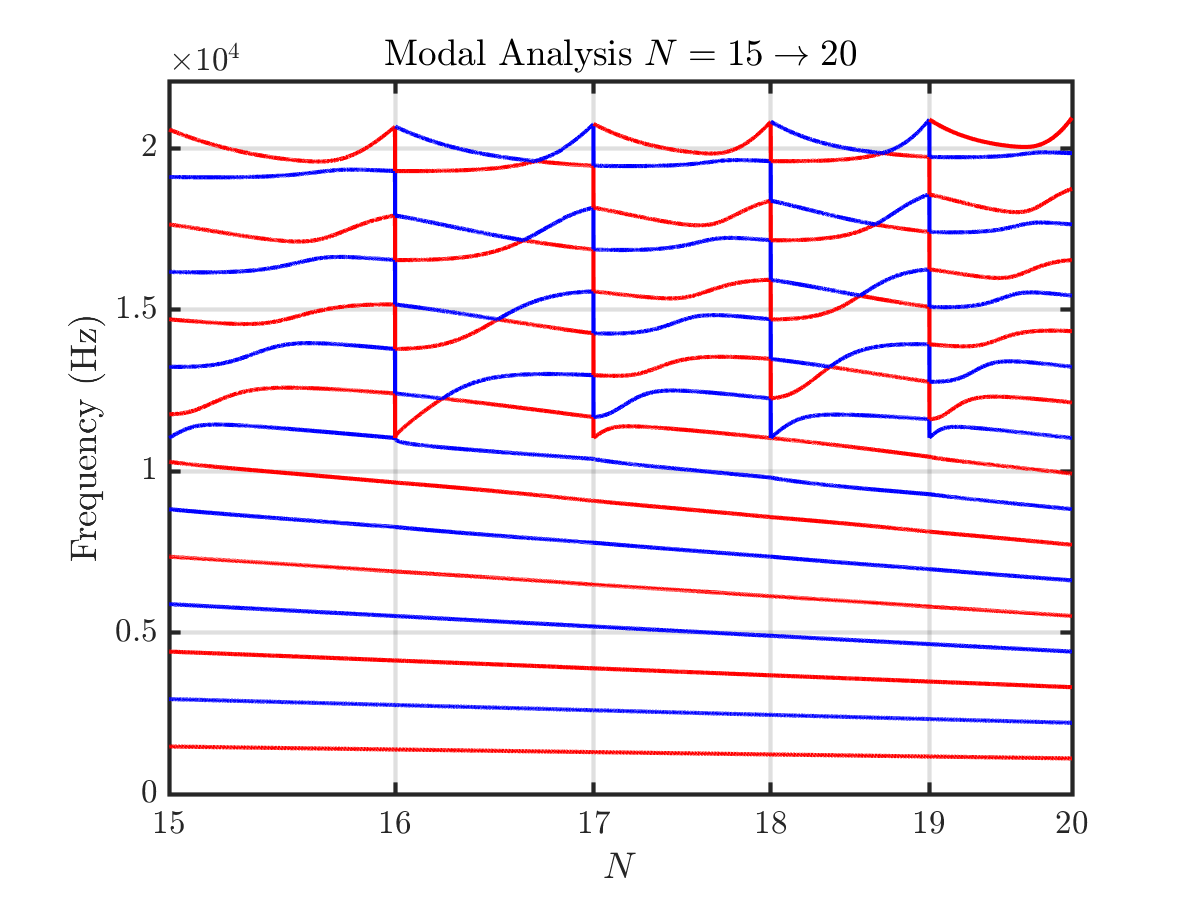
\includegraphics[width=0.45\textwidth]{modesAddPointsInCenter.eps}}}
    \hspace{0.05\textwidth}
    \subfloat[Spectrogram.]{\label{fig:cubSpecAddCenter}{ 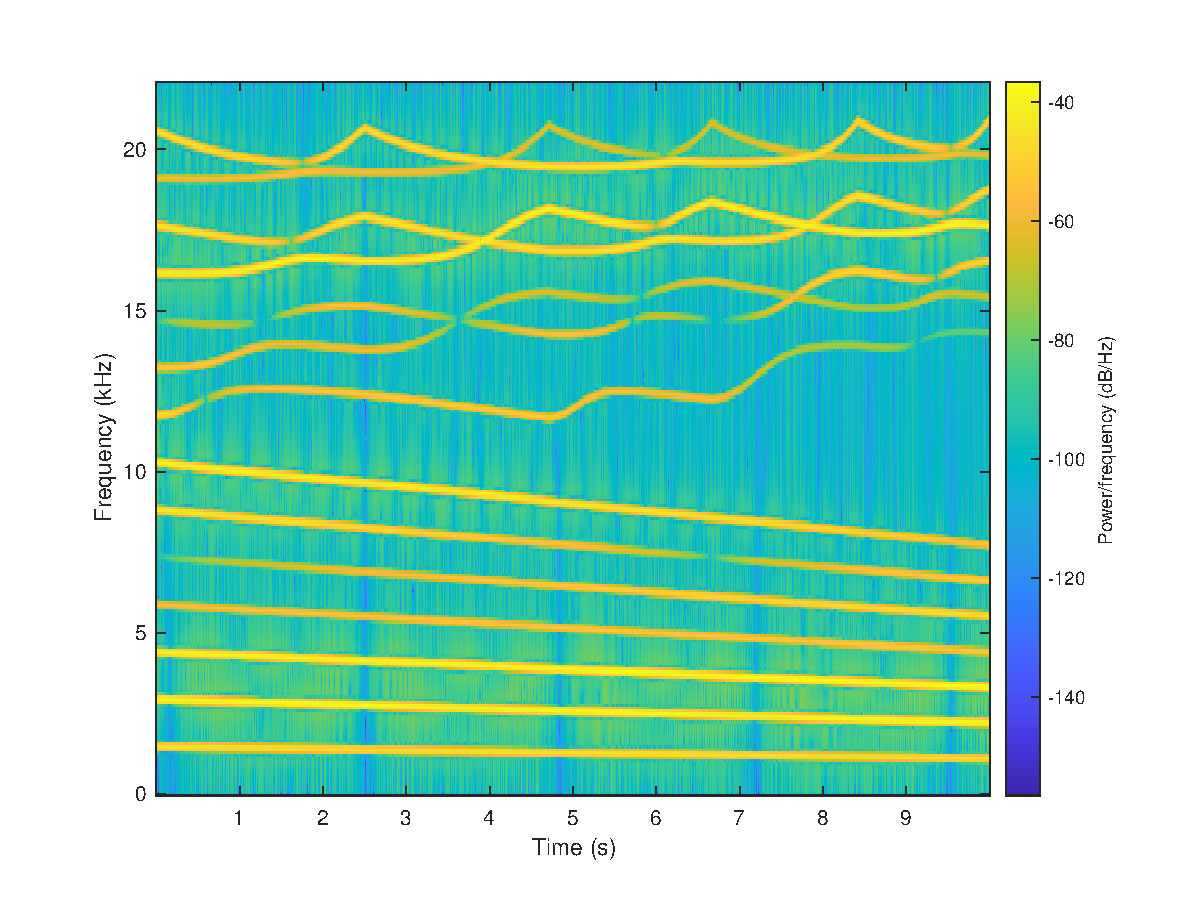
\includegraphics[width=0.45\textwidth]{specAddCenter.eps}}}
    \caption{Cubic Interpolation}\label{fig:cubAddInCenter}
\end{figure}
\subsubsection*{Two points on each side}
Alternatively, one can create a custom cubic interpolator for unequally spaced gridpoints using \eqref{eq:lagrangeForm}. If we want the number of points to the left and the right of $u_{M+1}$ to be the same we need to consider $u_M$ and $w_0$ and right of it are $w_1$ and $w_2$ (look at Figure \ref{fig:interpolatedZoom} for reference). Similar to section \ref{sec:lagrangeDeriv} we define the following 
\begin{equation}
    \begin{aligned}
     x_0 &= x_{u_{M}} = 0 \\
     x_1 &= x_{w_0} = \alpha \\
     x_2& = x_{w_1} = \alpha + 1 \\
     x_3 &= x_{w_2} = \alpha + 2,
    \end{aligned}
\end{equation}
and the $x$ that we're solving for is 
\begin{equation}
    x = x_{u_M+1} = 1.
\end{equation}
This results in the following interpolator:
\begin{equation}
    \mathcal{I}_3^\star = 
    \begin{bmatrix}
        \frac{\alpha - 1}{\alpha + 2} &
        \frac{\alpha + 1}{2}&
       (1-\alpha) &
       \frac{\alpha(\alpha - 1)}{2(\alpha + 2)}
    \end{bmatrix}\ .
\end{equation}
This results in the following $\mathbf{B}$ matrix:
\begin{equation}
    \mathbf{B}_3^\star = \begin{bmatrix}[cccc|cccc]
     & \ddots  &\ddots & & & & 0 & \\
       & 1 & 0 & 1 & & & & \\
      & & 1 & \frac{\alpha - 1}{\alpha + 2} & \frac{\alpha + 1}{2} & (1-\alpha) &\frac{\alpha(\alpha - 1)}{2(\alpha + 2)} \\ \cline{2-7}
      & \frac{\alpha(\alpha - 1)}{2(\alpha + 2)} & (1-\alpha) & \frac{\alpha + 1}{2} & \frac{\alpha - 1}{\alpha + 2} & 1 & & \\
         & & & &1 & 0 & 1  \\
         & 0 & &  &  &\ddots & \ddots &
    \end{bmatrix}
\end{equation}
\begin{figure}[h]
    \centering
    \subfloat[Modal analysis for alternative cubic interpolation.]{\label{fig:altCubModesAddInCenter}{ 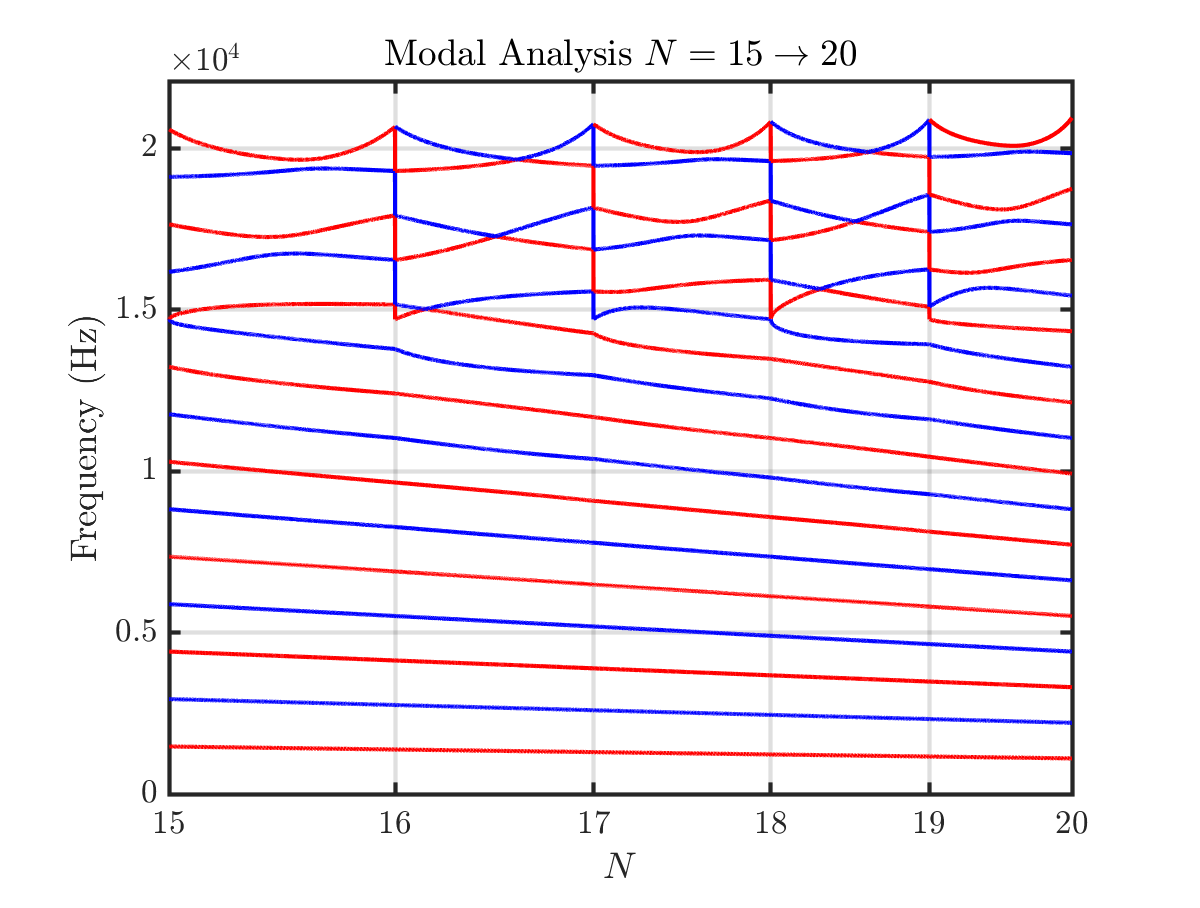
\includegraphics[width=0.45\textwidth]{modalAnalysisFigs/altCubicMid.eps}}}
    \hspace{0.05\textwidth}
    \subfloat[Spectrogram.]{\label{fig:altCubSpecAddCenter}{ 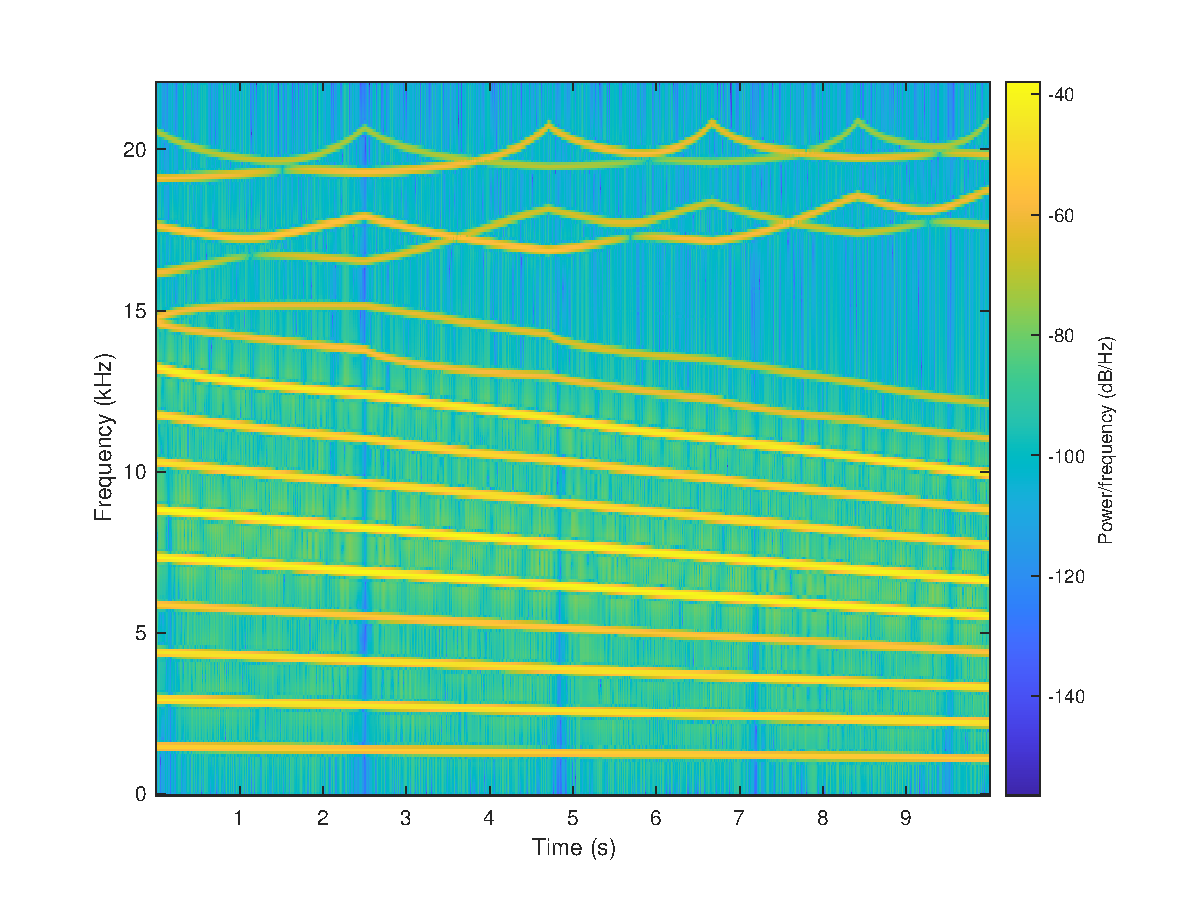
\includegraphics[width=0.45\textwidth]{modalAnalysisFigs/specAltCubicMid.eps}}}
    \caption{Alternative Cubic interpolation.}\label{fig:altCubAddInCenter}
\end{figure}
\subsubsection*{Same points for both virtual grid points}
As the results were still slightly unsatisfactory, a shifted version 

where for both virtual grid points, $u_{M-1}$, $u_{M}$, $w_0$ and $w_1$ were used.
\begin{equation}
    \mathbf{B}_3' = \begin{bmatrix}[cccc|cccc]
     & \ddots  &\ddots & & & & 0 & \\
       & 1 & 0 & 1 & & & & \\
      & & 1-\frac{\alpha(\alpha - 1)}{(\alpha + 1)(\alpha + 2)}& \frac{2(\alpha - 1)}{\alpha + 1} & \frac{2}{\alpha + 1} & -\frac{2(\alpha - 1)}{(\alpha + 1)(\alpha + 2)} \\ \cline{2-7}
      & & -\frac{2(\alpha - 1)}{(\alpha + 1)(\alpha + 2)}  & \frac{2}{\alpha + 1} &  \frac{2(\alpha - 1)}{\alpha + 1} &  1-\frac{\alpha(\alpha - 1)}{(\alpha + 1)(\alpha + 2)} & & \\
         & & & &1 & 0 & 1  \\
         & 0 & &  &  &\ddots & \ddots &
    \end{bmatrix}
\end{equation}
\subsubsection{Quartic interpolation}
Although with the alternative cubic interpolation approach there are two points on either side of the point we want to calculate, and in that sense symmetric, the distance from that point is not. We can take one extra point and create a quartic interpolator:
\begin{equation}
    \begin{aligned}
     x_0 &= x_{u_{M-1}} = 0 \\     
     x_1 &= x_{u_{M}} = 1 \\
     x_2 &= x_{w_0} = \alpha + 1 \\
     x_3& = x_{w_1} = \alpha + 2 \\
     x_4 &= x_{w_2} = \alpha + 3,
    \end{aligned}
\end{equation}
and the $x$ that we're solving for is 
\begin{equation}
    x = x_{u_M+1} = 2.
\end{equation}
This results in the following interpolator:
\begin{equation}
    \mathcal{I}_4 = 
    \begin{bmatrix}
        \frac{-\alpha(\alpha - 1)}{(\alpha + 2)(\alpha + 3)}
        &
        \frac{2(\alpha - 1)}{\alpha + 2}&
        1&
        \frac{-2(\alpha - 1)}{\alpha + 2}&
        \frac{\alpha(\alpha - 1)}{(\alpha + 2)(\alpha + 3)}
    \end{bmatrix}\ .
\end{equation}
and the following matrix
\begin{equation}
    \mathbf{B}_4 = \begin{bmatrix}[cccc|cccc]
     & \ddots  &\ddots & & & & 0 & \\
       & 1 & 0 & 1 & & & & \\
      & & 1 - \frac{\alpha(\alpha - 1)}{(\alpha + 2)(\alpha + 3)}& \frac{2(\alpha - 1)}{\alpha + 2} & 1 & -\frac{2(\alpha - 1)}{\alpha + 2} &\frac{\alpha(\alpha - 1)}{(\alpha + 2)(\alpha + 3)}\\ \cline{2-7}
      & \frac{\alpha(\alpha - 1)}{(\alpha + 2)(\alpha + 3)} & -\frac{2(\alpha - 1)}{\alpha + 2}  & 1 & \frac{2(\alpha - 1)}{\alpha + 2}  & 1 - \frac{\alpha(\alpha - 1)}{(\alpha + 2)(\alpha + 3)} & & \\
         & & & &1 & 0 & 1  \\
         & 0 & &  &  &\ddots & \ddots &
    \end{bmatrix}
\end{equation}

\begin{figure}[h]
    \centering
    \subfloat[Modal analysis for quartic interpolation.]{\label{fig:quartModesAddInCenter}{ 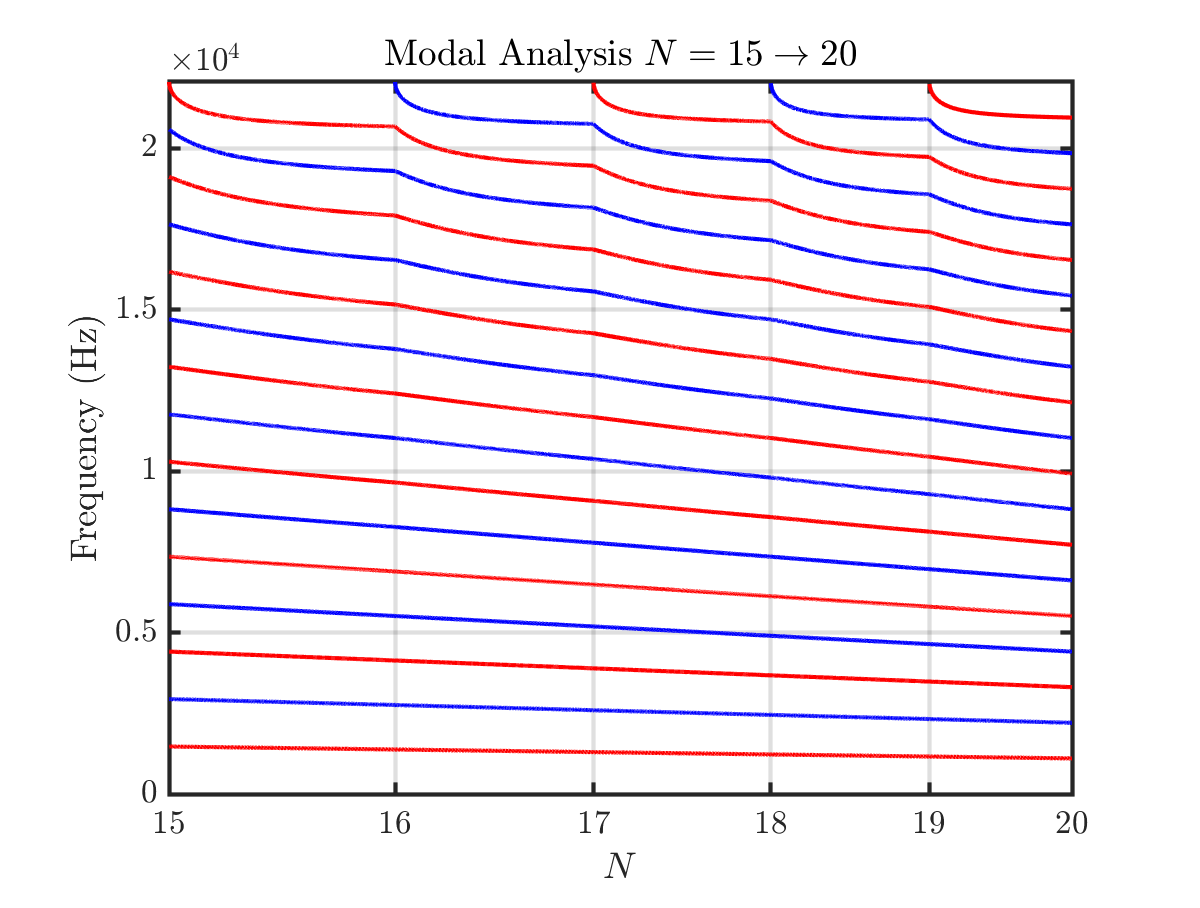
\includegraphics[width=0.45\textwidth]{modalAnalysisFigs/quarticMid.eps}}}
    \hspace{0.05\textwidth}
    \subfloat[Spectrogram of system wave excited with raised cosine when $N = 15$.]{\label{fig:quartSpecAddCenter}{ 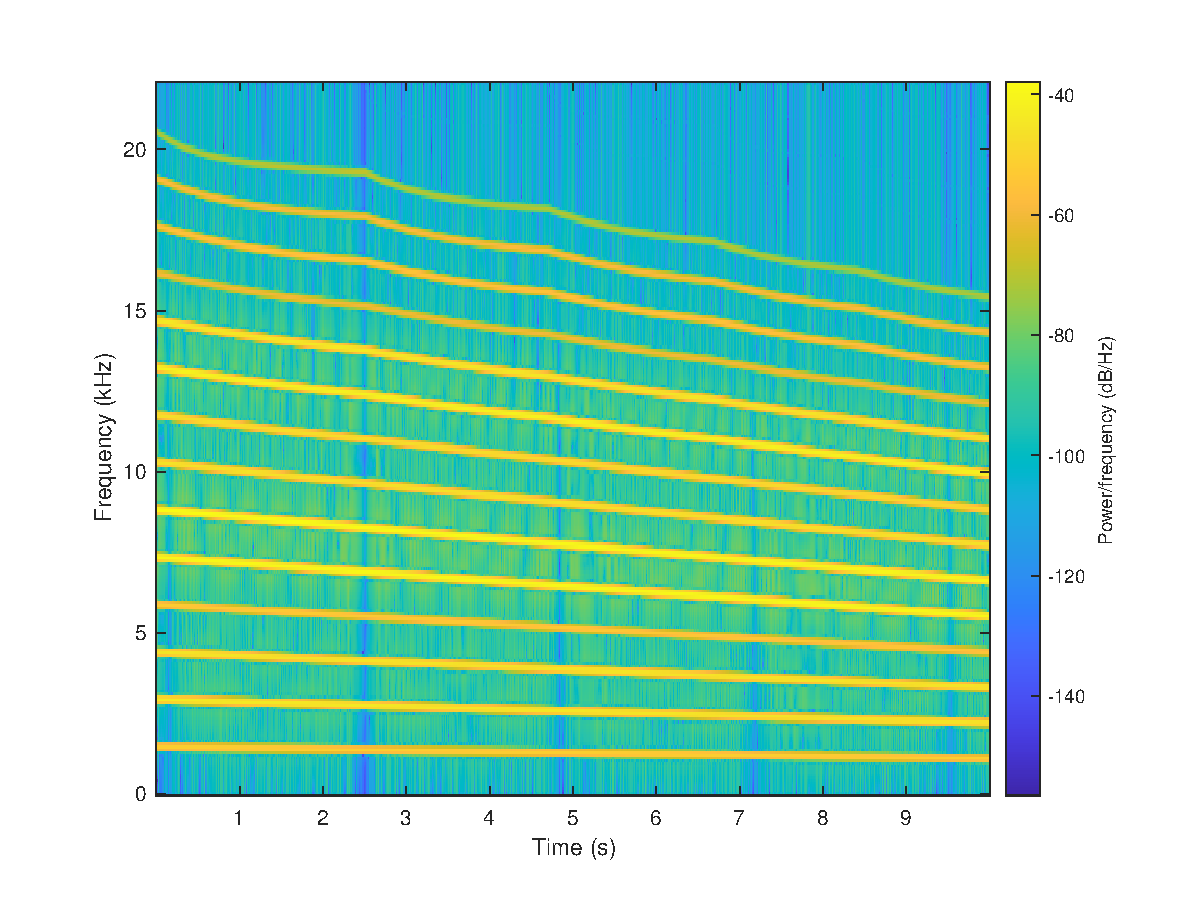
\includegraphics[width=0.45\textwidth]{modalAnalysisFigs/specQuarticMid.eps}}}
    \caption{Quartic interpolation.}\label{fig:quartSpecAddInCenter}
\end{figure}


The results for a system going linearly from $c=2940$ m/s ($N=15$) to $c = 2205$ m/s ($N=20$), can be found in Figure \ref{fig:addInCenter}. Figure \ref{fig:modesAddInCenter} shows a number of interesting things 
\begin{itemize}
    \item At every integer $N$, there are $N-1$ modes (related to the number of moving points at that point) that are integer multiples of the fundamental. This is expected and desired. However, due to the extra point used for overlap, an extra mode arises between the lower and the upper half of the harmonics. If the system is excited when the system has an integer $N$ (and $\alpha = 0$ in Eq. \eqref{eq:connectionInterpol}), this extra mode will not be excited due to the constraint of a rigid connection. 
    \item Modes lower than and equal to half the number of total modes follow a linear pattern down, whereas higher modes follow a ``squiggly" pattern upwards.
    \item Modal crossings can be seen when moving from an even to an odd $N$.
\end{itemize}
The spectrogram in Figure \ref{fig:specAddCenter} shows that excited modes follow the ``paths of least resistance" looking at Figure \ref{fig:modesAddInCenter}. The latter two points are an undesired behaviour. 

\SWcomment[Notes about what the expected / desired behaviour should be. -- or -- System Requirements
\begin{itemize}
    \item Smooth between different number-of-points-configurations
    \item Linearly down / up
\end{itemize}]
The following section goes into how to get closer to a desired behaviour.

\subsubsection{Deciding where to add / remove points}
Until now we have only looked at adding / removing points at the center of the string as in Eq. \eqref{eq:addingRemovingPoints}, i.e, alternating between the left and the right half. To get decrease of some of the undesired behaviour described above, such as ``squiggly" patterns for high modes and modal crossings. Trial and error showed that the closer the point add / remove location is to a boundary, the less this undesired behaviour shows up. The closest we can get to a boundary is to have $u$ be $N-1$ points (including the boundary) and $w$ two points, one moving, one boundary. If we then want to calculate the interpolated points using \eqref{eq:Av} we can extend the Dirichlet boundary condition in Eq. \eqref{eq:halfStringBoundaryCond} to the simply supported one
\begin{equation}
    w_{M_w} = \delta_{xx}w_{M_w} = 0, \quad \text{(Simply Supported)}
\end{equation}
to find the definition for $w_2^n$
\begin{equation}
    w_2^n = -w_0^n.
\end{equation}
This condition can be exploited to have less points interacting with each other (which probably caused the undesired behaviour described above). As $w_1$ is the boundary and thus excluded from the calculation we can build matrix $B_3'$
\begin{equation}
    \mathbf{B}_3' = 2\mathbf{I} + \lambda^2 \begin{bmatrix}[cccc|cc]
     & \ddots  &\ddots & & 0 & \\
       & 1 & -2 & 1 & & \\
      & \mathbf{A}_{1, 2}^\text{i}\alpha_\text{I} &\mathbf{A}_{1, 2}^\text{i}\beta_\text{I} + 1 &\mathbf{A}_{1, 2}^\text{i}\gamma_\text{I} -2 & \mathbf{A}_{1, 1}^\text{i}(\gamma_\text{I}-\alpha_\text{I})& \\ \cline{2-5}
      &\mathbf{A}_{2, 2}^\text{i}\alpha_\text{I} &\mathbf{A}_{2, 2}^\text{i}\beta_\text{I}&\mathbf{A}_{2, 2}^\text{i}\gamma_\text{I} & \mathbf{A}^\text{i}_{2,1}(\gamma_\text{I} - \alpha_\text{I})-2 & 
    \end{bmatrix}
\end{equation}
Analysing this using Eq. \eqref{eq:modalAnalysis} yields Figure \ref{fig:modesAddAtRightBound}.

\begin{figure}[h]
    \centering
    \subfloat[Modal analysis when points are added close at the boundary]{\label{fig:modesAddAtRightBound}{ 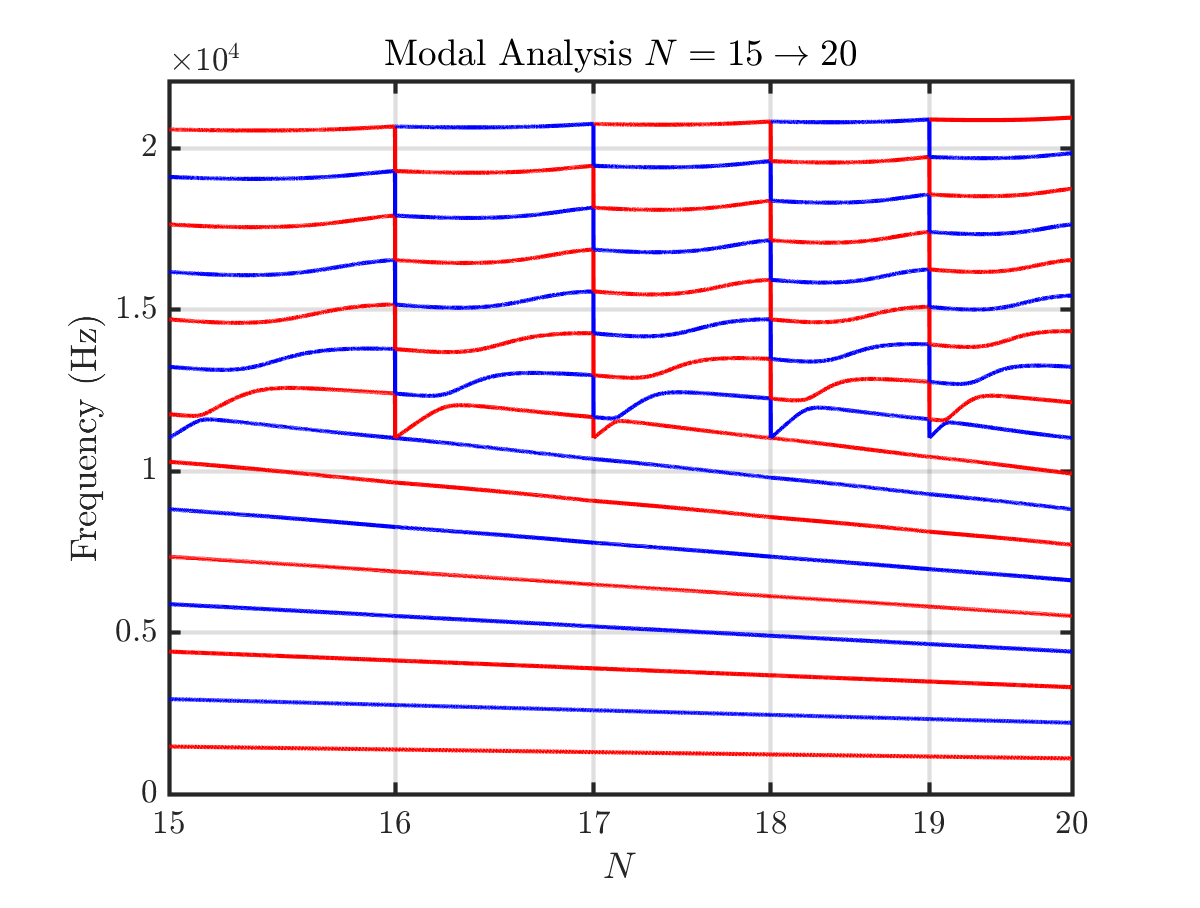
\includegraphics[width=0.45\textwidth]{modesAddPointsAtRightBound.eps}}}
    \hspace{0.05\textwidth}
    \subfloat[Spectrogram of system wave excited with raised cosine when $N = 15$.]{\label{fig:specAddCenter}{ 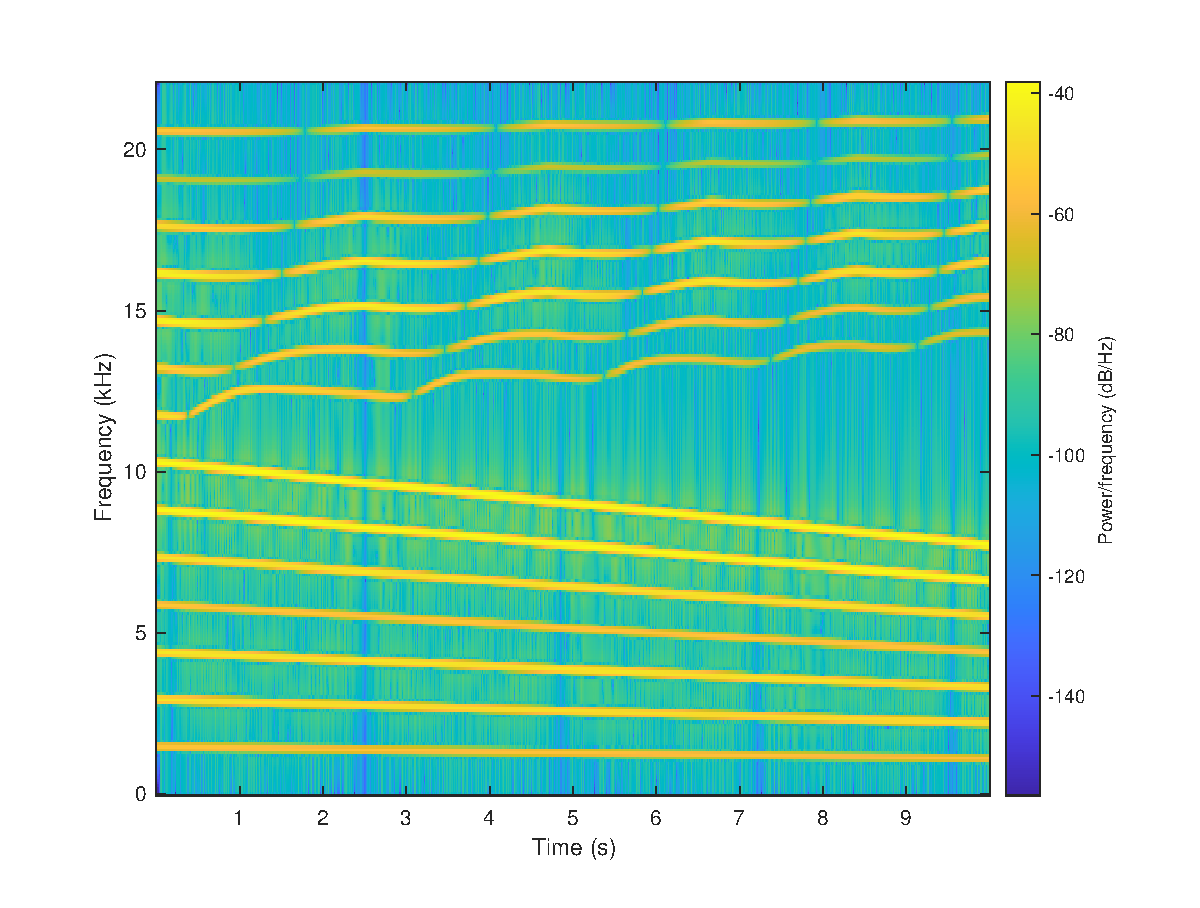
\includegraphics[width=0.45\textwidth]{specAddPointsAtRightBound.eps}}}
    \caption{1D wave going linearly from $c = 2940$ m/s ($N=15$) to $c =2205$ m/s ($N=20$). Points are added at the boundary.}\label{fig:addAtBoundary}
\end{figure}

\subsection{Energy}
As the quadratic interpolation has been chosen as the best interpolation technique (due to simplicity with small modal deviation), we continue with this.

To get the rate of change of the energy of $u$, we take the inner product of Eq. \eqref{eq:resultOneConnectedPoint1} with $\delta_{t\cdot}u$ over domain $\mathcal{D}_u = [0, M]$. As the right boundary is (partly) overlapping with the left boundary of $w$, a weighted inner product needs to be used
\begin{equation}\label{eq:weightedInnerProduct}
    \langle f,g \rangle_{\mathcal{D}}^{\epsilon_\text{l}, \epsilon_\text{r}}= \sum_{l = 1}^{N-1}hf_lg_l + \frac{\epsilon_\text{l}}{2}hf_0g_0 + \frac{\epsilon_\text{r}}{2}hf_Ng_N.
\end{equation}
Using Eq. \eqref{eq:weightedInnerProduct} with $\epsilon_\text{l} = 2$ (simply including that term into the sum) we get (a definition for $\epsilon_\text{r}$ will be defined later)
\begin{align*}
    \langle \delta_{t\cdot}u, \delta_{tt}u\rangle_{\mathcal{D}_u}^{\epsilon_\text{r}} &= c^2 \langle \delta_{t\cdot}u, \delta_{xx}u\rangle_{\mathcal{D}_u}^{\epsilon_\text{r}}\\
    \sum_{l = 0}^{M-1}h(\delta_{t\cdot}u_l^n)(\delta_{tt}u_l^n) + \frac{\epsilon_\text{r}}{2}h(\delta_{t\cdot}u_M^n)(\delta_{tt}u_M^n) &= c^2\left(\sum_{l = 0}^{M-1}h(\delta_{t\cdot}u_l^n)(\delta_{xx}u_l^n) + \frac{\epsilon_\text{r}}{2}h(\delta_{t\cdot}u_M^n)(\delta_{xx}u_M^n)\right)
\end{align*}
The total energy of $u$ is defined as
\begin{equation}
    \mathfrak{h}_u = \mathfrak{t}_u + \mathfrak{v}_u
\end{equation}
%
Taking the left-hand side and utilising identity (2.22a) from \cite{Bilbao2009} yields
\begin{equation}
    \delta_{t+}\mathfrak{t}_u = \delta_{t+}\left(\frac{1}{2}\sum_{l=0}^{M-1}h(\delta_{t-}u_l^n)^2 + \frac{\epsilon_\text{r}}{4}h(\delta_{t-}u_M^n)^2\right).
\end{equation}
The right-hand side is slightly more complicated. Moving it to the left-hand side and performing integration by parts we get:
\begin{equation*}
    c^2 \sum_{l=0}^{M-1} h (\delta_{t\cdot}\delta_{x+}u_l^n)(\delta_{x+}u_l^n) = \mathfrak{b}_u
\end{equation*}
and identity (2.22b) from \cite{Bilbao2009} to get 
\begin{equation}
    \delta_{t+}\left(\underbrace{\frac{c^2}{2} \sum_{l=0}^{M-1} h (\delta_{x+}u_l^n)(\delta_{x+}u_l^{n-1})}_{\mathfrak{v}_u}\right) = \mathfrak{b}_u
\end{equation}
where
\begin{align}
    \mathfrak{b}_u &= c^2\left((\delta_{t\cdot}u_M^n)\underbrace{(\delta_{x+}u_{M-1}^n)}_{\delta_{x-}u_M^n}- \underbrace{(\delta_{t\cdot}u_0^n)}_{= 0}(\delta_{x+}u_{-1}^n)+\frac{\epsilon_\text{r}}{2}h(\delta_{t\cdot}u_M^n)(\delta_{xx}u_M^n)\right)\nonumber\\
    & = c^2(\delta_{t\cdot}u_M^n)\left((\delta_{x-}u_M^n)+\frac{\epsilon_\text{r}}{2}h(\delta_{xx}u_M^n)\right)
\end{align}
%
We can do the same for Eq. \eqref{eq:resultOneConnectedPoint2} $\delta_{t\cdot}w$ over domain $\mathcal{D}_w = [0, M_w]$ and $\epsilon_\text{r} = 2$ to get 
\begin{equation}
    \delta_{t+}\mathfrak{t}_w = \delta_{t+}\left(\frac{1}{2}\sum_{l=1}^{M_w} h(\delta_{t-}w_l^n)^2 + \frac{\epsilon_\text{l}}{4}h(\delta_{t-}w_0^n)^2\right),
\end{equation}
and 
\begin{equation}
    \delta_{t+}\left(\underbrace{\frac{c^2}2 \sum_{l=1}^{M_w} h (\delta_{x+}w_l^n)(\delta_{x+}w_l^{n-1})}_{\mathfrak{v}_w}\right) = \mathfrak{b}_w
\end{equation}
where
\begin{align}
    \mathfrak{b}_w &= c^2\left(-(\delta_{t\cdot}w_0^n)\underbrace{(\delta_{x-}w_{1}^n)}_{\delta_{x+}w_0^n}- \underbrace{(\delta_{t\cdot}w_{M_w}^n)}_{= 0}(\delta_{x-}w_{M_w+1}^n)+\frac{\epsilon_\text{l}}{2}h(\delta_{t\cdot}w_0^n)(\delta_{xx}w_0^n)\right)\nonumber\\
    &= c^2(\delta_{t\cdot}w_0^n)\left(-(\delta_{x+}w_0^n)+\frac{\epsilon_\text{l}}{2}h(\delta_{xx}w_0^n)\right)
\end{align}
The total (rate of change of) energy will then become 
\begin{equation}
    \delta_{t+}\left(\mathfrak{h}_u + \mathfrak{h}_w\right) = \mathfrak{b}_u + \mathfrak{b}_w
\end{equation}
where the boundary terms on the right hand side of the equation can be seen as the potential energy between the two inner boundaries. 

We can now find the values of $\epsilon_\text{r}$ and $\epsilon_\text{l}$. When $\alpha = 0$ we know that all energy should be contained within $\mathfrak{h}_u$ and $\mathfrak{h}_w$ and $\mathfrak{b}_u + \mathfrak{b}_w = 0$. 
\begin{equation}\label{eq:innerBoundEnergyCalcIntermediate}
    \mathfrak{b}_u + \mathfrak{b}_w = c^2\left[(\delta_{t\cdot}u_M^n)\left((\delta_{x-}u_M^n)+\frac{\epsilon_\text{r}}{2}h(\delta_{xx}u_M^n)\right) + (\delta_{t\cdot}w_0^n)\left(-(\delta_{x+}w_0^n)+\frac{\epsilon_\text{l}}{2}h(\delta_{xx}w_0^n)\right)\right]= 0
\end{equation}
Furthermore, the rigid connection imposed on the inner boundaries when $\alpha = 0$ means that $\delta_{t\cdot}u_M^n = \delta_{t\cdot}w_0^n$. Eq. \eqref{eq:innerBoundEnergyCalcIntermediate} can be rewritten to 
\begin{equation*}
    c^2(\delta_{t\cdot}u_M^n)\left((\delta_{x-}u_M^n)+\frac{\epsilon_\text{r}}{2}h(\delta_{xx}u_M^n) -(\delta_{x+}w_0^n)+\frac{\epsilon_\text{l}}{2}h(\delta_{xx}w_0^n)\right)= 0
\end{equation*}
which is true if $\delta_{t\cdot}u_M^n=0$, $c = 0$ or the rest is $0$. As the first two solutions are trivial, we continue with the latter and expand
\begin{equation}\label{eq:intermediateEnergyEq}
    \frac{1}{h}\left(u_M^n - u_{M-1}^n +\frac{\epsilon_\text{r}}{2}(u_{M+1}^n-2u_M^n+u_{M-1}^n) -w_1^n + w_0^n + \frac{\epsilon_\text{l}}{2}(w_1^n - 2 w_0^n + w_{-1}^n) \right)= 0,
\end{equation}
after which the definitions for the virtual grid points ($u_{M+1}^n$ and $w_{-1}^n$) can be filled in. Using 
\begin{equation}
    \Iterm = \frac{\alpha - 1}{\alpha + 1}
\end{equation}
and multiplying Eq. \eqref{eq:intermediateEnergyEq} by $2h$ yields
\begin{equation}
    (2+\epsilon_\text{r}(\Iterm - 2) + \epsilon_\text{l})u_M^n + (-2 + \epsilon_\text{r} - \epsilon_\text{l}\Iterm) u_{M-1}^n + (2+\epsilon_\text{l}(\Iterm - 2) + \epsilon_\text{r})w_0^n + (-2 + \epsilon_\text{l} - \epsilon_\text{r}\Iterm) w_1^n = 0.
\end{equation}
In order for this equality to hold, all coefficients need to be 0, as the grid values change value per definition. It can be shown that the coefficients are identical, apart from a sign inversion. Assuming that $\epsilon_\text{r} = \epsilon_\text{l}$ (as the connection is symmetric anyway) we can set one of the coefficients to 0, and solve for $\epsilon$ 
\begin{align*}
    2 + \epsilon(\Iterm-2) + \epsilon &= 0\\
    \epsilon = - \frac{2}{\Iterm - 1}
\end{align*}
Expanding $\Iterm$ yields
\begin{align*}
    \epsilon &= -\frac{2}{\frac{\alpha - 1}{\alpha + 1} - 1}\\
    \epsilon &= -\frac{2(\alpha + 1)}{\alpha - 1 - (\alpha + 1)}\\
\end{align*}
and finally yielding the following definition for $\epsilon$
\begin{equation}
    \epsilon = \alpha + 1.
\end{equation}
This is also inline with the amount of ``space'' one grid point takes. A perfect overlap ($\alpha = 0$) scales the kinetic energy of $u_M$ and $w_0$ by 0.5 obtaining the full kinetic energy for that grid location when added together. As $\alpha \rightarrow 1$ these points are not scaled at all, i.e, $\epsilon \rightarrow 2$. In this case, the boundary terms actually reduce to the potential energy between the inner boundaries. 
\begin{align*}
    \mathfrak{b}_u + \mathfrak{b}_w &=c^2\Big[(\delta_{t\cdot}u_M^n)\big((\delta_{x-}u_M^n)+h(\delta_{xx}u_M^n)\big)+(\delta_{t\cdot}w_0^n)\big(-(\delta_{x+}w_0^n)+h(\delta_{xx}w_0^n)\big)\Big]
    \\
    &= \frac{c^2}{h}\Big((\delta_{t\cdot}u_M^n)(u_M^n - u_{M-1}^n + \Iterm u_M^n + w_0^n - \Iterm w_1^n - 2u_M^n + u_{M-1}^n) \\
    &\qquad+ (\delta_{t\cdot}w_0^n)(-w_1^n+w_0^n + w_1^n-2w_0^n-\Iterm u_{M-1}^n + u_M^n + \Iterm w_0^n)\Big)\\
    \xLeftrightarrow{\mystrut\ \Iterm = 0\ } &= \frac{c^2}{h}\Big((\delta_{t\cdot}u_M^n)(w_0^n - u_M^n )+ (\delta_{t\cdot}w_0^n)(-w_0^n+ u_M^n)\Big)\\
    &= \frac{c^2}{h}\Big((\delta_{t\cdot}u_M^n - \delta_{t\cdot}w_0^n)(w_0^n - u_M^n)\Big)\\
    \xLeftrightarrow{\mystrut\ w_0^n = u_{M+1}^n\ }&= -c^2h(\delta_{t\cdot}\delta_{x+}u_M^n)(\delta_{x+}u_M^n)
\end{align*}
which, again using Eq. (2.22b) from \cite{Bilbao2009} can be rewritten to
\begin{equation}
    \mathfrak{b}_u+\mathfrak{b}_w = -\frac{c^2}{2}\delta_{t+}\big(h(\delta_{x+}u_M^n)(\delta_{x+}u_M^{n-1})\big),  
\end{equation}
and is reduced to the potential energy between the inner boundaries. 

To summarise, the total energy of the system can be calculated using
\begin{equation}
    \delta_{t+}\left(\mathfrak{h}_u + \mathfrak{h}_w\right) = \mathfrak{b}_u + \mathfrak{b}_w
\end{equation}
with 
\begin{equation}
    \begin{aligned}
    \mathfrak{b}_u &= c^2(\delta_{t\cdot}u_M^n)\left((\delta_{x-}u_M^n)+\frac{\epsilon}{2}h(\delta_{xx}u_M^n)\right) \quad \text{and}\\
    \mathfrak{b}_w &= c^2(\delta_{t\cdot}w_0^n)\left(-(\delta_{x+}w_0^n)+\frac{\epsilon}{2}h(\delta_{xx}w_0^n)\right)
    \end{aligned}
\end{equation}
and $\epsilon = \alpha + 1$.


\subsection{Displacement correction}
When the wavespeed is increased and points are removed, it is not necessarily true that $u_M = w_0$ at the time of removal and the rigid connection in \eqref{eq:rigid} is violated. On top of the virtual grid point ``generation'' from the interpolation described above, one could add a connection force that is dependent on how close the inner boundaries $u_M$ and $w_0$ are.

We can extend \eqref{eq:systemHalfStrings} to have a spring force between $u_M$ and $w_0$ as
\begin{equation}\label{eq:dispCorrSyst}
    \begin{cases}
        \delta_{tt}u^n &= c^2\delta_{xx}u^n + J(x_{u_M})F\\
        \delta_{tt}w^n &= c^2\delta_{xx}w_0^n - J(x_{w_0})F
    \end{cases}
\end{equation}
with 
\begin{equation}\label{eq:corrForceNoDamp}
    F = \beta \mu_{t\cdot}\eta^n.
\end{equation}
Here,
\begin{equation}\label{eq:etaCorrDef}
    \eta^n \triangleq w_0^n - u_M^n
\end{equation}
is the difference in displacement between the inner boundaries
and $\beta = \beta(\alpha)$ 
acts as a spring coefficient that is a function of the distance between the inner boundaries along the grid, i.e., $\alpha$. Furthermore, the centred temporal averaging operator $\mu_{t\cdot}$ is used in \eqref{eq:corrForceNoDamp} to ensure stability \cite{Bilbao2009}.

We then continue by finding a definition for $\beta$ that is inversely proportional to $\alpha$, i.e., the smaller $\alpha$ is the higher the `correction' effect, ideally approaching an infinite stiffness, or rigid connection, when $\alpha = 0$ and no stiffness when $\alpha \rightarrow 1$. This can be achieved by defining $\beta = \beta(\alpha)$ as
\def\plusEps{+ \epsilon}
% \def\plusEps{};
\def\alfPlusEps{(\alpha \plusEps)}
% \def\alfPlusEps{\alpha}
\begin{equation}\label{eq:betaDef}
    \beta = \frac{1 - \alpha}{\alpha \plusEps},
\end{equation}
with $0<\epsilon \ll 1$ to prevent a division by 0. It will be shown that when calculating the force after expansion, a division by 0 can be prevented and $\epsilon = 0$ will still yield a defined solution. We can observe that when $\alpha = 0$ and the correction effect needs to be at a maximum, $\beta\rightarrow \infty$. When $\alpha \rightarrow 1$, $\beta \rightarrow 0$.

We can also add a damping term to \eqref{eq:corrForceNoDamp} which is also scaled by $\beta$ as
\begin{equation}\label{eq:corrForce}
    F = \beta \left(\mu_{t\cdot}\eta^n +\sigma_0\delta_{t\cdot}\eta^n \right),
\end{equation}
where $\sigma_0$ is the damping coefficient. Then, we can solve for $\eta^{n+1}$ 
\begin{align}
    F &= \beta\left(\frac{1}{2}\left(\eta^{n+1}+\eta^{n-1}\right) + \frac{\sigma_0}{2k}\left(\eta^{n+1}-\eta^{n-1}\right)\right)\nonumber\\
    F&= \left(\frac{\beta (1 + \sigma_0/k)}{2}\right)\eta^{n+1} + \left(\frac{\beta (1 - \sigma_0/k)}{2}\right) \eta^{n-1}\nonumber\\
    \xLeftrightarrow{\mystrut\ \text{Eq. \eqref{eq:betaDef}}\ } \quad \eta^{n+1} &= \left(\frac{2
    \alfPlusEps}{(1+\sigma_0/k)(1-\alpha)}\right)F - \underbrace{\frac{1-\sigma_0/k}{1+\sigma_0/k}}_{r}\eta^{n-1}.\label{eq:etaSolut1}
\end{align}
Using superscript $\text{I}$ to denote an intermediate state describing of $u^{n+1}_M$ and $w^{n+1}_0$ without the connection force (see \eqref{eq:resultOneConnectedPoint}), we also know, through Eq. \eqref{eq:etaCorrDef}, that 

\begin{align}
    \eta^{n+1} &= w_0^\text{I}-\frac{k^2}{h}F-\left(u_M^\text{I}+\frac{k^2}{h}F\right)\nonumber\\
    \eta^{n+1} &= w_0^\text{I} - u_M^\text{I} - \frac{2k^2}{h}F,\label{eq:etaNext}
\end{align}
which can be set equal to \eqref{eq:etaSolut1} and solved for $F$ according to 

\begin{align*}
    \left(\frac{2
    \alfPlusEps}{(1+\sigma_0/k)(1-\alpha)}\right)F - r \eta^{n-1} &= w_0^{I} - u_M^{I}- \frac{2k^2}{h}F\\
    \left(\frac{2h
    \alfPlusEps + 2k^2(1+\sigma_0/k)(1-\alpha)}{h(1+\sigma_0/k)(1-\alpha)}\right)F &= w_0^{I} - u_M^{I}+r\eta^{n-1}\\
    F &= \left(w_0^{I} - u_M^{I}+r\eta^{n-1}\right)\left(\frac{h(1+\sigma_0/k)(1-\alpha)}{2h \alfPlusEps + 2k^2(1+\sigma_0/k)(1-\alpha)}\right).
\end{align*}
It is clear now that no matter the value of $\alpha$, no division by 0 will occur, so $\epsilon = 0$ is still defined. The final equation for $F$ can thus be written as
\begin{equation}\label{eq:finalForce}
    F = \left(w_0^{I} - u_M^{I}+r\eta^{n-1}\right)\underbrace{\left(\frac{h(1+\sigma_0/k)(1-\alpha)}{2h\alpha + 2k^2(1+\sigma_0/k)(1-\alpha)}\right)}_{\Psi}.
\end{equation}
This can then be filled into \eqref{eq:dispCorrSyst} and used to get $u_M^{n+1}$ and $w_0^{n+1}$ respectively. \SWcomment[Using $\alpha = 0$ and $\sigma_0 = 0$ as a test case to see what would happen to the scheme at the inner boundaries when they perfectly overlap (and without damping, just restoring force), we get that $r = 1$ and \eqref{eq:finalForce} becomes
\begin{align*}
    F &= \left(w_0^{I} - u_M^{I}+\eta^{n-1}\right)\left(\frac{h}{2k^2}\right)\\
    \xLeftrightarrow{\mystrut\ \text{Eq. \eqref{eq:etaNext}}\ } \quad F &= \left(\eta^{n+1} + \frac{2k^2}{h}F + \eta^{n-1}\right)\left(\frac{h}{2k^2}\right)\\
    F - F &= \eta^{n+1} + \eta^{n-1}\\
    2\mu_{t\cdot}\eta^n &= 0\\
    \mu_{t\cdot}\eta^n &= 0
\end{align*}
showing that when $\alpha = 0$, the $\eta^n$ should be 0 and thus boils down to a rigid connection.]

As the intermediate states are as defined as \eqref{eq:resultOneConnectedPoint} (the scheme without the correction effect), %with virtual gridpoints $u_{M+1}^n \triangleq w_1^n$ and $w_{-1}^n \triangleq u_{M-1}^n$, 
and %knowing that $\lambda = 1$ at all times, we can simplify this to
% \begin{subequations}
%     \begin{numcases}{}
%         u^{I}_M = u_{M-1}^n+u_{M+1}^n- u_M^{n-1}\\
%         w^{I}_0 = w_{-1}^n+w_1^n - w_0^{n-1}
%     \end{numcases}
% \end{subequations}
% Then, 
using \eqref{eq:etaCorrDef} for $\eta^{n-1}$ yields
\begin{align*}
    F &= \Psi\left(w_{-1}^n + w_1^n - w_0^{n-1} - u_{M+1}^n-u_{M-1}^n + u_M^{n-1} + r (w_0^{n-1} - u_M^{n-1})\right)\\
    F&= \Psi\left(w_{-1}^n + w_1^n - (1-r)w_0^{n-1} - u_{M+1}^n-u_{M-1}^n + (1-r)u_M^{n-1}\right).
\end{align*}
Substituting this into \eqref{eq:dispCorrSyst} and evaluated at the inner boundaries yields
\begin{align*}
    u^{n+1}_M &= u_{M-1}^n + u_{M+1}^n - u_M^{n-1} + \underbrace{\frac{\Psi k^2}{h}}_{\psi}\left(w_{-1}^n + w_1^n - (1-r)w_0^{n-1} - u_{M+1}^n-u_{M-1}^n + (1-r)u_M^{n-1}\right)\\
    u^{n+1}_M &= (1-\psi)u_{M-1}^n + (1-\psi)u_{M+1}^n - (1-\psi(1-r))u_M^{n-1} + \psi\left(w_{-1}^n + w_1^n - (1-r)w_0^{n-1}\right)
\end{align*}
and
\begin{align*}
    w^{n+1}_0 &= w_{-1}^n + w_{1}^n - w_0^{n-1} - \psi\left(w_{-1}^n + w_1^n - (1-r)w_0^{n-1} - u_{M+1}^n-u_{M-1}^n + (1-r)u_M^{n-1}\right)\\
    w^{n+1}_0 &= (1-\psi)w_{-1}^n + (1-\psi)w_{1}^n - (1-\psi(1-r))w_0^{n-1} + \psi\left(u_{M+1}^n+u_{M-1}^n - (1-r)u_M^{n-1}\right)
\end{align*}
Then, filling in the definitions for the virtual using quadratic interpolation:
\def\Iterm{\mathcal{A}}
\begin{subequations}\label{eq:quadraticDef}
    \begin{align}
        &\begin{aligned}\label{eq:calcUMP1}
            u_{M+1}^n = \Iterm u_{M}^n + w_0^n - \Iterm w_1^n
        \end{aligned}\\
        &\ \ \begin{aligned}\label{eq:calcWM1}
            w_{-1}^n
            =-\Iterm u_{M-1}^n + u_{M}^n+ \Iterm w_{0}^n.
        \end{aligned}
    \end{align}
\end{subequations}
with 
\begin{equation}
    \Iterm = \frac{\alpha - 1}{\alpha + 1}
\end{equation}
yields
\begin{align}
    &\begin{aligned}
    u^{n+1}_M =\ & (1-\psi)u_{M-1}^n + (1-\psi)\left(\Iterm u_{M}^n + w_0^n - \Iterm w_1^n\right) - (1-\psi(1-r))u_M^{n-1} \\
    &+ \psi\left(-\Iterm u_{M-1}^n + u_{M}^n+ \Iterm w_{0}^n + w_1^n - (1-r)w_0^{n-1}\right)
    \end{aligned}\nonumber\\
    &\begin{aligned}
    u_M^{n+1} =\ & (1-\psi - \psi\Iterm)u_{M-1}^n + (\Iterm-\psi \Iterm + \psi)u_M^n + (1-\psi + \psi\Iterm) w_0^n - (\Iterm-\psi \Iterm - \psi) w_1^n\\
    &- (1 - \psi + \psi r) u_M^{n-1} - (\psi - \psi r) w_0^{n-1}\end{aligned}\label{eq:uMnp1expanded}
\end{align}
and
\begin{align}
    &\begin{aligned}
    w^{n+1}_0 =\ & (1-\psi)w_1^n + (1-\psi)\left(-\Iterm u_{M-1}^n + u_M^n + \Iterm w_0^n\right) - (1-\psi(1-r))w_0^{n-1}\\
    &+ \psi\left(\Iterm u_M^n + w_0^n-\Iterm w_1^n + u_{M-1}^n - (1-r)u_M^{n-1}\right)
    \end{aligned}\nonumber\\
    &\begin{aligned}
    w_0^{n+1} =\ & (1-\psi - \psi\Iterm)w_1^n + (\Iterm-\psi \Iterm + \psi)w_0^n + (1-\psi + \psi\Iterm) u_M^n - (\Iterm-\psi \Iterm - \psi) u_{M-1}^n\\
    &- (1 - \psi + \psi r) w_0^{n-1} - (\psi - \psi r) u_M^{n-1}\end{aligned}
    \label{eq:w0np1expanded} 
\end{align}
% \begin{align*}
%     & \begin{cases}
        
%     \end{cases}
% \end{align*}

\subsubsection{Modal Analysis}
Due to the damping that is present in the system, it needs to be written in one-step form. Recalling \eqref{eq:uVecDef} we can write write \eqref{eq:dispCorrSyst} in vector-matrix form
\begin{equation}\label{eq:formForOneStep}
    \A \U^{n+1} = \B \U^n + \C\U^{n-1}
\end{equation}
and rewrite to one-step form as
\begin{equation}\label{eq:oneStepForm}
    \underbrace{\begin{bmatrix}
        \U^{n+1}\\
        \U^n
    \end{bmatrix}}_{\mathbf{W}^{n+1}} = 
    \underbrace{\begin{bmatrix}
        \A^{-1}\B & \A^{-1}\C\\
        \I & \mathbf{0}
    \end{bmatrix}}_{\Q}
    \underbrace{\begin{bmatrix}
        \U^n\\
        \U^{n-1}
    \end{bmatrix}}_{\mathbf{W}^n}
\end{equation}
Using Eqs. \eqref{eq:uMnp1expanded} and \eqref{eq:w0np1expanded} we get the following definitions for the matrices
\begin{equation}
    \A = \I
\end{equation}
\begin{equation}
    \mathbf{B} = \begin{bmatrix}[cccc|cccc]
     & \ddots  &\ddots & & & & 0 & \\
       & 1 & 0 & 1 & & & & \\
      & & (1-\psi-\psi \Iterm) & (\Iterm-\psi\Iterm+\psi) & (1-\psi+\psi\Iterm) & -(\Iterm-\psi\Iterm - \psi) & \\ \cline{2-7}
      & & -(\Iterm-\psi\Iterm-\psi) & (1-\psi+\psi\Iterm) & (\Iterm-\psi\Iterm+\psi) & (1-\psi-\psi\Iterm) & & \\
         & & & &1 & 0 & 1  \\
         & 0 & &  &  &\ddots & \ddots &
    \end{bmatrix}
\end{equation}
or decomposed in \eqref{eq:quadMat} and the correction force
\begin{equation}
    \mathbf{B} = \mathbf{B}_2 + \mathbf{B}_\text{c}
\end{equation}
where
\begin{equation}
    \mathbf{B}_c = \psi \cdot \begin{bmatrix}[cccc|cccc]
     & 0  & & & & & 0 & \\
       & & & & & & & \\
      & & -(1+\Iterm) & (1-\Iterm) & (\Iterm-1) & (\Iterm + 1) & \\ \cline{2-7}
      & & (\Iterm+1) & (\Iterm-1) & (1-\Iterm) &-(1+\Iterm) & & \\
         & & & & & &  \\
         & 0 & &  &  & & 0 &
    \end{bmatrix}
\end{equation}
and 
\begin{equation}
    \C = \begin{bmatrix}[cccc|cccc]
     & \ddots  & & & & & \mathbf{0} & \\
       & 0 & -1 & 0 & & & & \\
      & &  & -(1-\psi + \psi r) & -(\psi - \psi r)  &  & \\ \cline{2-7}
      & &  & -(\psi - \psi r)& -(1-\psi + \psi r)  &  & & \\
         & & & & 0 & -1 & 0 \\
         & \mathbf{0} & &  &  & & \ddots &
    \end{bmatrix}
\end{equation}
Alternatively, and possibly more straightforward, is to expand the forces in system \eqref{eq:dispCorrSyst} directly. 
% \begin{equation}
%     \begin{cases}
%         \delta_{tt}u^n &= c^2\delta_{xx}u^n + J(x_{u_M})\frac{\beta}{2}(\eta^{n+1} + \eta^{n-1} + \sigma_0/k (\eta^{n+1} - \eta^{n-1}))\\
%         \delta_{tt}w^n &= c^2\delta_{xx}w_0^n - J(x_{w_0})\frac{\beta}{2}(\eta^{n+1} + \eta^{n-1} + \sigma_0/k (\eta^{n+1} - \eta^{n-1}))
%     \end{cases}
% \end{equation}
% and
Recalling $\U$ from \eqref{eq:uVecDef} (of size $\mathcal{M} = M+M_w$) and, (very important) including the virtual grid point definitions encapsulated in $\B_2$, we can rewrite the system to
\begin{equation}
    \I\U^{n+1} = \B_2\U^n - \I\U^{n-1} + (\J\boldsymbol{\eta})\frac{\beta k^2}{2}\left((1+\sigma_0/k)\U^{n+1} + (1-\sigma_0/k)\U^{n-1}\right)
\end{equation}
where 
\begin{equation}
    \J = [\mathbf{0}_{M-1}, 1/h, -1/h, \mathbf{0}_{M_w-1}]^T
\end{equation}
where $\mathbf{0}_i$ is a row-vector of zeros with length $i$ and
\begin{equation}
    \boldsymbol{\eta} = [\mathbf{0}_{M-1}, -1, 1, \mathbf{0}_{M_w-1}].
\end{equation}
vectorising the effect of \eqref{eq:etaCorrDef} on $\U$. Note that as $\J$ is a column vector and $\boldsymbol{\eta}$ a row vector, the multiplication of the two yields an $\mathcal{M}\times\mathcal{M}$ matrix.

Then refactoring to the form in \eqref{eq:formForOneStep} and using identity matrix $\I$ with size $\mathcal{M} \times \mathcal{M}$ yields the following matrices
% \begin{equation}
%     \underbrace{\left(\I - \frac{\beta k^2 (1+\sigma_0/k)}{2}\J\boldsymbol{\eta}\right)}_{\A}\U^{n+1} = \underbrace{\mathbf{B}_2}_{\B}\U^n +\underbrace{\left(- \I - \frac{\beta k^2 (1-\sigma_0/k)}{2}\J\boldsymbol{\eta}\right)}_{\C} \U^{n-1}
% \end{equation}

\begin{equation}
    \A = \I - \frac{\beta k^2 (1+\sigma_0/k)}{2}\J\boldsymbol{\eta}, \qquad \B = \mathbf{B}_2, \qquad \text{and} \qquad \C = -\left(\I - \frac{\beta k^2 (1-\sigma_0/k)}{2}\J\boldsymbol{\eta}\right)
\end{equation}
Although substituting these definitions into \eqref{eq:oneStepForm} gives an identical result to the matrix definitions above (comparisons show a difference between the $\Q$ matrices around machine precision), $\beta$ can still go to infinity. In this case, $\epsilon \neq 0$ in \eqref{eq:betaDef}. 

\subsection{Stiff string}
To prove that this technique also works with more complicated schemes, we can apply the above to the stiff string with the following scheme
\begin{equation}
    \delta_{tt}u = c^2\delta_{xx}u - \kappa^2\delta_{xxxx}u
\end{equation}
where $\kappa = \sqrt{EI/\rho A}$ with Young's modulus $E$ and moment of inertia $I$. The difference with the 1D-wave equation is the stiffness term containing a fourth order spatial derivative. This requires an extra virtual grid point to be calculated at the boundaries. For the outer boundaries we choose simply supported conditions according to
\begin{equation}
    u_0 = w_{M_w} = \delta_{xx}u_0 =  \delta_{xx}w_{M_w} = 0.
\end{equation}
The points needed at the other boundaries are calculated below. 

We start by (again) connecting $u_{M}^n$ and $w_0^n$ using a rigid connection using \eqref{eq:rigid} yielding the following system:
\begin{equation}
    \begin{cases}
        \delta_{tt}u_l^n = c^2\delta_{xx}u_l^n-\kappa^2\delta_{xxxx}u_l^n + J(x_{u_M})F\\
        \delta_{tt}w_l^n = c^2\delta_{xx}w_l^n -\kappa^2\delta_{xxxx}w_l^n - J(x_{w_0})F.
    \end{cases} 
\end{equation}
If we expand the spatial derivative operators and using the concept of weight ratio due to the overlap (see Appendix \ref{app:overlap}) we get
\begin{equation}\label{eq:systemHalfStiffStrings}
    \begin{cases}
        \delta_{tt}u_M^n = \frac{c^2}{h^2}(2u_{M-1}^n-u_M^n)-\frac{\kappa^2}{h^4}(2u_{M-2}^n - 8u_{M-1}^2+6u_M^n) + \frac{1}{h}F\\
        \delta_{tt}w_0^n = \frac{c^2}{h^2}(2w_1^n-w_0^n)-\frac{\kappa^2}{h^4}(2w_2^n - 8w_1^2+6w_0^n) - \frac{1}{h}F.
    \end{cases} 
\end{equation}
Again, because \eqref{eq:rigid} is true, $\delta_{tt}u_M = \delta_{tt}w_0$ and by setting the equations in \eqref{eq:systemHalfStiffStrings} equal to each other we can solve for $F$
\begin{gather}
    \frac{c^2}{h^2}(2u_{M-1}^n- 2u_M^n)-\frac{\kappa^2}{h^4}(2u_{M-2}^n - 8u_{M-1}^n + 6 u_M^n) + \frac{1}{h}F =  \nonumber\\
    \frac{c^2}{h^2}(2w_1^n - 2w_0^n) -\frac{\kappa^2}{h^4}(2w_2^n - 8w_1^n + 6w_0^n) - \frac{1}{h}F\nonumber\\
    \frac{2}{h}F = \frac{c^2}{h^2}(2w_1^n - 2w_0^n-2u_{M-1}^n+2u_M^n)-\frac{\kappa^2}{h^4}(2w_2^n - 8w_1^n + 6w_0^n - 2u_{M-2}^n + 8u_{M-1}^n - 6u_M^n)\nonumber\\
    F = h\frac{c^2}{h^2}(w_1^n-u_{M-1}^n)-h\frac{\kappa^2}{h^4}(w_2^n-4w_1^n+4u_{M-1}^n-u_{M-2}^n).
\end{gather}
If we add this to the respective equations in \eqref{eq:systemHalfStiffStrings} and expand the acceleration term to get the following updates
\begin{equation}\label{eq:systemHalfStiffStrings}
    \begin{cases}
        u_M^{n+1} = 2u_M^n - u_M^{n-1}+ \lambda^2(u_{M-1}^n-2u_M^n+w_1^n)-\mu^2(u_{M-2}^n - 4u_{M-1}^2+6u_M^n-4w_1^n+w_2^n)\\
        w_0^{n+1} = 2w_0^n - w_0^{n-1}+ \lambda^2(u_{M-1}^n-2w_0^n+w_1^n)-\mu^2(u_{M-2}^n - 4u_{M-1}^2 + 6w_0^n - 4w_1^2 + w_2^n),
    \end{cases} 
\end{equation}
which are (again) equivalent expressions for the connected point. 

\SWcomment[Along the same lines\footnote{might have to prove something here}] we can find updates for $u_{M-1}^n$ and $w_1^n$, which -- through the fourth-order spatial derivative -- are now also affected by the state of the other string:
\begin{equation}\label{eq:systemHalfStiffStrings}
    \begin{cases}
        u_{M-1}^{n+1} = 2u_{M-1}^n - u_{M-1}^{n-1}+ \lambda^2(u_{M-2}^n-2u_{M-1}^n+u_M^n)-\mu^2(u_{M-3}^n - 4u_{M-2}^n+6u_{M-1}^n-4u_M^n+w_1^n)\\
        w_1^{n+1} = 2w_1^n - w_1^{n-1}+ \lambda^2(w_0^n-2w_1^n+w_2^n)-\mu^2(u_{M-1}^n - 4w_0^n + 6w_1^n - 4w_2^n + w_3^n).
    \end{cases} 
\end{equation}
\section{Adding an overlap}\label{app:overlap}
Another, slightly trickier, setup could be that the left string has an extra point at its right side to cause some overlap. This might come in handy later if we want to interpolate the forces between the strings for better quality. We can then apply two rigid connections to the overlapping points
\begin{equation}\label{eq:doubleRigid}
    \begin{aligned}
    u_{M-1}^n &= w_0^n,\\
    u_M^n &= w_1^n.
    \end{aligned}
\end{equation}
See Figure \ref{fig:overlap} for clarification. 

\begin{figure}[h]
    \centering
    \subfloat[Overlapped points.]{\label{fig:overlapFull}{ 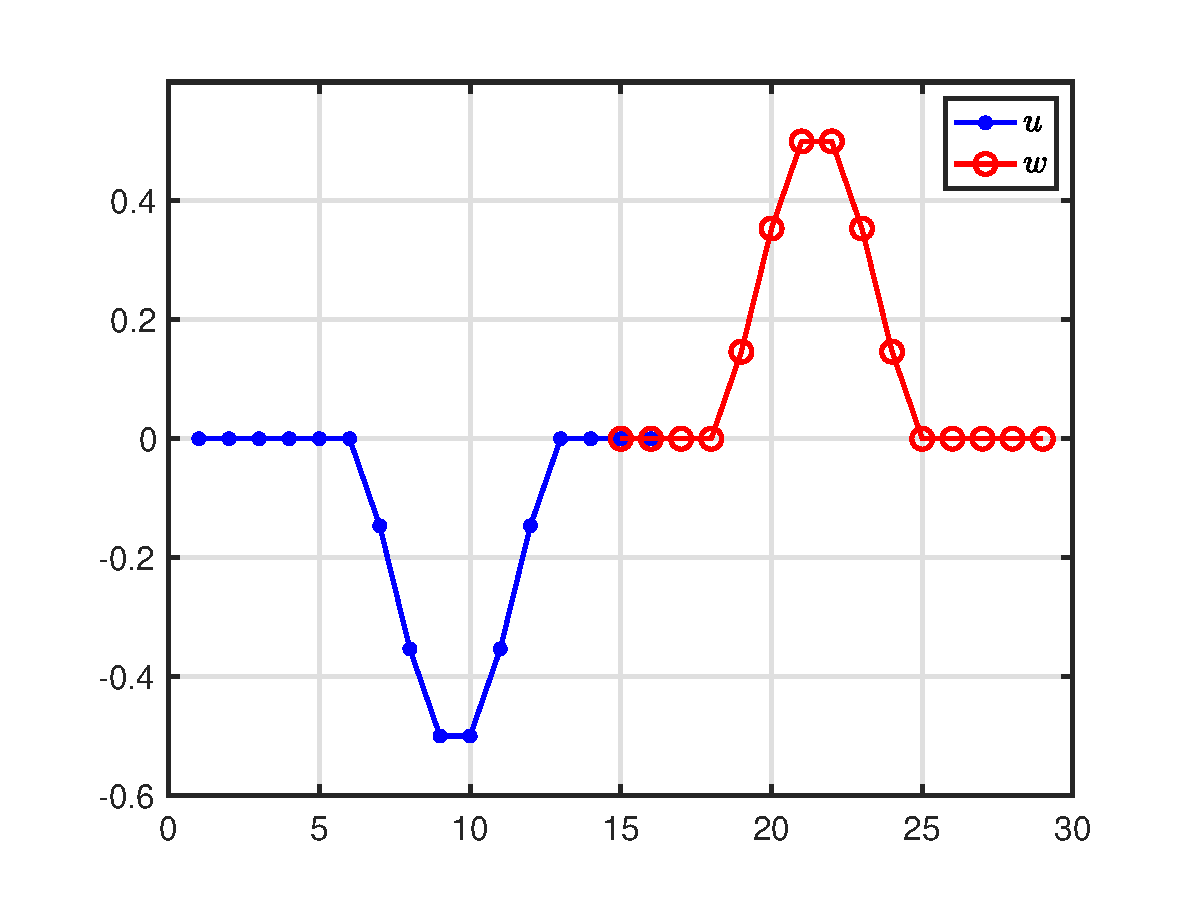
\includegraphics[width=0.5\textwidth]{twoStringsOverlap.eps}}}
    \subfloat[Zoomed. Note that the overlapping points should always have the same state, but they have been pulled apart for clarity.]{\label{fig:overlapZoom}{ 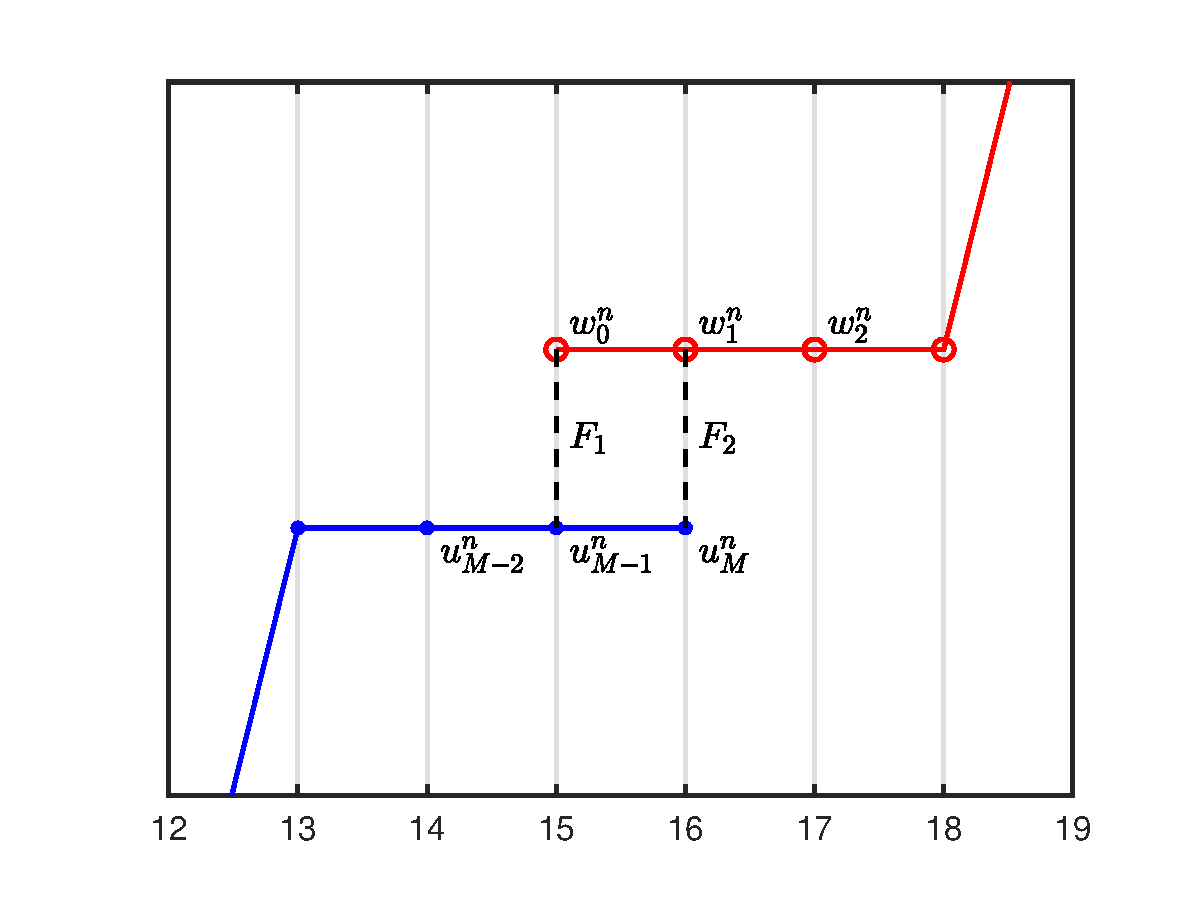
\includegraphics[width=0.5\textwidth]{overlapForces.eps}}}
    \caption{}\label{fig:overlap}
\end{figure}

As an overlap happens, the string is ``heavier" at this point if we keep the same physical parameters. However, in reality, the string is equally heavy everywhere. As shown in Figure \ref{fig:overlapZoom}, the overlapping points ($u_{M-1}^n, u_{M}^n, w_0^n$ and $w_1^n$) have to be made twice as light as their non-overlapping counterparts. From their perspective, $u_{M-2}^n$ and $w_2^n$ are twice as heavy when compared to themselves. Imagine changing the material density of these to double of what they usually are. This will change the wave speed according to:
\begin{equation}
    c^2 = T/\rho A \quad \xRightarrow[]{\ 2\rho\ }\quad c^2 = T/2\rho A \quad \Rightarrow \quad 2c^2 = T/\rho A.
\end{equation}

For the overlapping points, we will now have the following update equations
\begin{equation}\label{eq:updateOverlap}
    \begin{cases}
        u_{M-1}^{n+1} = 2u_{M-1}^n - u_{M-1}^{n-1} + \lambda^2 (2u_{M-2}^n - 2u_{M-1}^n + u_{M}^n) + \frac{k^2}{h}F_1\\
        u_{M}^{n+1} = 2u_{M}^n - u_{M}^{n-1} + \lambda^2 (u_{M-1}^n - 2u_M^n) + \frac{k^2}{h}F_2\\
        w_0^{n+1} = 2w_0^n-w_0^{n-1} + \lambda^2 (w_1^n-2w_0^n) - \frac{k^2}{h}F_1\\
        w_1^{n+1} = 2w_1^n-w_1^{n-1} + \lambda^2 (w_0^n-2w_1^n+2w_2^n) - \frac{k^2}{h}F_2
    \end{cases}
\end{equation}
\SWcomment[One would think that some scaling also needs to happen for $u_{M-1}^n$ in the update equation for $u_{M-2}^{n+1}$ and $w_1^n$ in $w_2^n$, but as we will see shortly, this is not necessary.]
This concept of a weight ratio also automatically happened in the previous case because of the Neumann boundary condition.

Recalling \eqref{eq:doubleRigid}, we can then solve for $F_1$ and $F_2$ in the same way as before. 

\begin{align}
    2u_{M-1}^n - u_{M-1}^{n-1} + \lambda^2(2u_{M-2}^n-2u_{M-1}^n + u_{M}^n) + \frac{k^2}{h} F_1 &=
    2w_0^n - w_0^{n-1} + \lambda^2(w_1^n-2w_0^n) - \frac{k^2}{h} F_1\nonumber\\
    \frac{2k^2}{h}F_1 &= \lambda^2(- 2u_{M-2}^n)\nonumber\\
    F_1 &= -h \frac{c^2}{h^2}(u_{M-2}^n)
\end{align}
and 
\begin{align}
    2u_M^n - u_M^{n-1} + \lambda^2(u_{M-1}^n-2u_M^n) + \frac{k^2}{h} F_2 &=
    2w_1^n - w_1^{n-1} + \lambda^2(w_0^n-2w_1^n+2w_2^n) - \frac{k^2}{h} F_2\nonumber\\
    \frac{2k^2}{h}F_2 &= \lambda^2(2w_2^n)\nonumber\\
    F_2 &= h \frac{c^2}{h^2}(w_2^n).
\end{align}

When filled into the update equations in \eqref{eq:updateOverlap} we get 
\begin{equation}\label{eq:updateOverlap}
    \begin{cases}
        u_{M-1}^{n+1} = 2u_{M-1}^n - u_{M-1}^{n-1} + \lambda^2 (u_{M-2}^n - 2u_{M-1}^n + u_{M}^n)\\
        u_{M}^{n+1} = 2u_{M}^n - u_{M}^{n-1} + \lambda^2 (u_{M-1}^n - 2u_M^n + w_2^n)\\
        w_0^{n+1} = 2w_0^n-w_0^{n-1} + \lambda^2 (w_1^n-2w_0^n+u_{M-2}^n)\\
        w_1^{n+1} = 2w_1^n-w_1^{n-1} + \lambda^2 (w_0^n-2w_1^n+w_2^n).
    \end{cases}
\end{equation}
Here, similarly to \eqref{eq:resultOneConnectedPoint}, $w_2^n$ and $u_{M-2}^n$ in the updates for $u_M^{n+1}$ and $w_0^{n+1}$ respectively act as virtual grid points.
Now we can also see why as scaling for overlapping points $u_{N-1}^n$ and $w_1^n$ in the updates for $u_{M-2}^{n+1}$ and $w_2^{n+1}$ are not necessary.

\subsubsection{Preliminary tests..}
...show instability...

\subsection{Energy}
For the kinetic energy, we now have to add a scaling with $0.5$, not only to the last point, but also to the rest of the overlapping ones:
\begin{align}
    \mathfrak{t}_u &= \sum_{l=0}^{M-2}   h(\delta_{t-}u_l^n)^2 + \frac{h}{2}(\delta_{t-}u_{M-1}^n)^2 + \frac{h}{2}(\delta_{t-}u_M^n)^2\\
    \mathfrak{t}_w &= \sum_{l=2}^{M}h(\delta_{t-}w_l^n)^2 + \frac{h}{2}(\delta_{t-}w_0^n)^2 + \frac{h}{2}(\delta_{t-}w_1^n)^2
\end{align}
\begin{align}
    \mathfrak{v}_u &= \frac{c^2}{2}\sum_{l=0}^{M-2} h(\delta_{x+}u_l^n)(\delta_{x+}u_l^{n-1}) + c^2\frac{h}{4} (\delta_{x+}u_{M-1}^n)(\delta_{x+}u_{M-1}^{n-1})\\
    \mathfrak{v}_w &= \frac{c^2}{2}\sum_{l=1}^{M-1} h(\delta_{x+}w_l^n)(\delta_{x+}w_l^{n-1}) + c^2\frac{h}{4} (\delta_{x+}w_0^n)(\delta_{x+}w_0^{n-1})
\end{align}

\section{Dirichlet Condition (Stefan)}

Consider a domain of length $L$, and grid spacing $h = ck$ (so, right at the Courant limit). Set $N = floor(L/h)$. Set the grid locations to be
\begin{equation}
x_{0} = 0,\quad x_{1} = h,\quad\hdots,\quad x_{N-1} = (N-1)h, \quad x_{N} = L = (N+\alpha)h
\end{equation}
where $0\leq \alpha\leq 1$. The final grid point lies directly on the boundary. 

Under Dirichlet conditions, we set $u_{0} = 0$ and $u_{N} = 0$. The Laplacian takes the form\footnote{\SWcomment[$\frac{2}{\alpha+1} = \frac{2}{\alpha+\SWcomment[2]}+\frac{2}{(\alpha+2)(\alpha+1)}$]}
\begin{eqnarray}
    \delta_{xx}u_{1}&=& \frac{1}{h^2}\left(u_{2}-2u_{1}\right)\\
    \delta_{xx}u_{l} &=& \frac{1}{h^2}\left(u_{l+1}-2u_{l}+u_{l-1}\right)\qquad 2\leq l\leq N-2\\
    \delta_{xx}u_{N-1} &=& \frac{1}{h^2}\left(\frac{2}{\alpha+2}u_{N-2}-\frac{2}{\alpha+1}u_{N-1}\right)\label{eq:uNmin1}
\end{eqnarray}
and thus, in matrix form, 
\begin{equation}
{\bf D}_{xx} = \frac{1}{h^2} 
    \begin{bmatrix}
    -2 & 1 & & &\\
    1 & -2 & 1 & &\\
     & \ddots & \ddots & \ddots & \\
     && 1 & -2 & 1\\
     &&& \frac{2}{\alpha+2} & -\frac{2}{\alpha+1}\\
    \end{bmatrix}
\end{equation}
The scheme, as a whole, then looks like
\begin{equation}
    \delta_{tt}{\bf u}^{n} = c^2{\bf D}_{xx}{\bf u}^{n}
\end{equation}
Define the matrix ${\bf P}$ as
\begin{equation}
    {\bf P} = {\rm diag}\left(1,1,\hdots,\frac{\alpha+2}{2}\right)
\end{equation}
Then ${\bf P D}_{xx}$ is now symmetric. 

Left-multiplying the scheme by ${\bf P}$ and then taking the inner product with $\delta_{t\cdot}{\bf u}$ then gives a conserved energy. Notice that this reduces to the usual case when $\alpha = 0$. 

\subsection{Taylor series expansion (Silvin)}
To get to the coefficients for $u_{N-2}$ and $u_{N-1}$ in \eqref{eq:uNmin1} we use a Taylor series expansion around the grid point $N-1$. To start, it is easiest to assume an expansion around 0 and then apply it to a different location. 

Suppose we have three grid locations $x_{-1} = -h, x_0 = 0$ and $x_1 = h (\alpha + 1)$ and their function values $u_{-1}, u_0$ and $u_1$. We then want to find an approximation $L = \frac{\partial^2 u}{\partial x^2} + O(h)$ (where $O(h)$ describes the order of the error) of the form
%
\begin{equation}\label{eq:formL}
    L = a_{-1}u_{-1} + a_0 u_0 + a_1 u_1
\end{equation}
%
where the coefficients $a_{-1}, a_0$ and $a_1$ depend on $\alpha$. \SWcomment[I suppose in the regular case ($\alpha = 0$) the coefficients end up being $a_{-1} = 1/h^2$, $a_0 = -2/h^2$ and $a_1 = 1/h^2$.] To find these coefficients we perform a Taylor series expansion. First we need to assume for a continuous function $u(x)$ that $u_{-1} = u(x_{-1}), u_0 = u(x_0)$ and $u_1 = u(x_1)$. We can then approximate this function $u$ around location $x_0 (=0)$ as 
\begin{equation}\label{eq:taylor}
    u(x) = u(0) + \frac{du(0)}{dx}x + \frac{1}{2}\frac{d^2u(0)}{dx^2}x^2 + O(x^3).
\end{equation}
Here, $O(x^3)$ describes the order of the error (or the collective error term with order of $x^3$).

We can then fill in the values of $x_{-1}$ and $x_1$ above ($u(x_0) = u(0)$) to get
\begin{align}
    u(-h) &= u(0) + \frac{du(0)}{dx}(-h) + \frac{1}{2}\frac{d^2u(0)}{dx^2}(-h)^2 + O(h^3)\nonumber\\
    &= u(0) - h \frac{du(0)}{dx} + \frac{h^2}{2}\frac{d^2u(0)}{dx^2} + O(h^3),
\end{align}
and 
\begin{align}
    u(h(\alpha+1)) &= u(0) + \frac{du(0)}{dx}(h(\alpha+1)) + \frac{1}{2}\frac{d^2u(0)}{dx^2}(h(\alpha+1))^2 + O(h^3)\nonumber\\
    &= u(0) + h(\alpha+1) \frac{du(0)}{dx} + \frac{h^2(\alpha+1)^2}{2}\frac{d^2u(0)}{dx^2} + O(h^3).
\end{align}
The goal is then to solve for $\frac{d^2u(0)}{dx^2}$ as this is what we want to approximate in \eqref{eq:1Dwave}. We want to get rid of the first-order derivative term so we can perform the following addition
\begin{align}
    u(-h) + \frac{u(h(\alpha+1))}{\alpha+1} &= \left(1+\frac{1}{\alpha+1}\right)u(0) + \left(-h + \frac{h(\alpha+1)}{\alpha + 1}\right)\frac{du(0)}{dx} + \left(\frac{h^2}{2} + \frac{h^2(\alpha+1)^2}{2(\alpha+1)}\right)\frac{d^2u(0)}{dx^2}+ O(h^3)\nonumber\\
    \frac{(\alpha+1)u(-h) + u(h(\alpha+1))}{\alpha+1}&= \left(\frac{\alpha + 2}{\alpha + 1}\right) u(0) + \left(\frac{h^2 + h^2(\alpha+1)}{2}\right)\frac{d^2u(0)}{dx^2}+ O(h^3)\nonumber\\
    \!\!\!\!\!\!\!\!\!\!\!\!\!\!\!\!\!\!\!\!\!\!\!\!\!\!\!\!\!\!\!\!\!\!\!\frac{(\alpha+1)u(-h) - (\alpha+2)u(0)+ u(h(\alpha+1))}{\alpha+1}&= \left(\frac{h^2(\alpha+2)}{2}\right)\frac{d^2u(0)}{dx^2}+ O(h^3)\nonumber\\
    L = \frac{d^2u(0)}{dx^2} + O(h) &= \frac{2((\alpha+1)u(-h) - (\alpha+2) u(0) + u(h(\alpha+1)))}{h^2(\alpha+2)(\alpha+1)}.
\end{align}
Note that due to a division with $h^2$ the order of the error is $O(h)$ rather than $O(h^3)$.
The coefficients in \eqref{eq:formL} are then as follows:
\begin{equation}
    a_{-1} = \frac{2}{h^2(\alpha+2)}, \quad a_0 = -\frac{2}{h^2(\alpha+1)}, \quad \text{and} \quad a_1 = \frac{2}{h^2(\alpha+2)(\alpha+1)}.
\end{equation}
% \subsubsection{Using forward and backward approximations for the first order derivatives}
% Then, we need to approximate the derivatives in \eqref{eq:taylor}. When $x = x_{-1}$, the first derivative is defined as (backwards)
% \begin{equation}
%     \frac{du(0)}{dx} \approx \frac{u(0) - u(-h)}{h} = \frac{u_0 - u_{-1}}{h}\ ,
% \end{equation}
% and when $x = x_{1}$ it is (forwards)
% \begin{equation}
%     \frac{du(0)}{dx} \approx \frac{u(h(\alpha+1)) - u(0)}{h(\alpha+1)} = \frac{u_1 - u_{0}}{h(\alpha + 1)}\ .
% \end{equation}
% From these we can get a definition of the second derivative
% \begin{align}
%     \frac{d^2u(0)}{dx^2} &= \frac{\frac{u_1 - u_0}{h(\alpha+1)} - \frac{u_0 - u_{-1}}{h}}{\frac{h(\alpha+1) + h}{2}}\nonumber\\
%     &= \frac{\left(\frac{2(u_1-u_0-(\alpha+1)u_0+(\alpha+1)u_{-1})}{h(\alpha+1)}\right)}{h(\alpha+2)}\nonumber\\
%     &= \frac{2(u_1-(\alpha+2)u_0+(\alpha+1)u_{-1})}{h^2(\alpha+2)(\alpha+1)}\label{eq:secondOrderTaylor}
% \end{align}

% we can fill in the values of $x_{-1}$ and $x_1$ above ($u(x_0) = u_0$) to get
% \begin{align}
%     u(-h) &= u_0 + \frac{u_0 - u_{-1}}{h}(-h) + \frac{1}{2} \frac{2(u_1-(\alpha+2)u_0+(\alpha+1)u_{-1})}{h^2(\alpha+2)(\alpha+1)} (-h)^2\nonumber\\
%     &= u_{-1} + \frac{u_1-(\alpha+2)u_0+(\alpha+1)u_{-1}}{(\alpha+2)(\alpha+1)}\nonumber\\
% &= \left(1+\frac{1}{\alpha+2}\right)u_{-1} - \frac{1}{\alpha+1} u_0 + \frac{1}{(\alpha+2)(\alpha+1)}u_1,
% \end{align}
% and
% \begin{align}
%     u(h(\alpha+1)) &= u_0 + \frac{u_1-u_0}{h}(h(\alpha+1)) + \frac{1}{2} \frac{2(u_1-(\alpha+2)u_0+(\alpha+1)u_{-1})}{h^2(\alpha+2)(\alpha+1)} (h(\alpha+1))^2\nonumber\\
%     &= u_0 + (\alpha + 1) (u_1 - u_0) + \frac{(\alpha+1)(u_1-(\alpha+2)u_0+(\alpha+1)u_{-1})}{\alpha + 2}\nonumber\\
%     &= \frac{(\alpha + 1)^2}{\alpha + 2} u_{-1} - (2(\alpha+1) - 1)u_0 + \left((\alpha+1) + \frac{\alpha+1}{\alpha+2}\right)u_1.
% \end{align}
% We can then use these terms to approximate the second derivative
% \begin{align}
%     L &= \frac{1}{h^2}\big[u(-h)-2u(0)+u(h(\alpha+1))\big]\\
%     &= \frac{1}{h^2}\left[\left(\frac{(\alpha+2) + 1 + (\alpha+1)^2}{\alpha+2}\right)u_{-1} - \left(\frac{1}{\alpha+1}+ 2(\alpha+1) - 1 + 2\right)u_0 + \left(\frac{1 + (\alpha+2)(\alpha+1)^2 + (\alpha+1)^2}{(\alpha+2)(\alpha+1)}\right)u_1\right]
% \end{align}
% \SWcomment[However, here it seems that if $\alpha = 0$, the approximation becomes $L = \frac{1}{h^2}(2u_{-1} - 4u_0 + 2u_1)$, i.e., twice what it is supposed to be..]
% \subsubsection{Using the centered approximation for the first order derivative}
% Instead, we can approximate the first derivative with a centered approximation:
% \begin{equation}
%     \frac{du(0)}{dx} \approx \frac{u(h(\alpha+1) - u(-h))}{h + h(\alpha+1)} = \frac{u_1 - u_{-1}}{h(\alpha + 2)}\ .
% \end{equation}
% In this case (and using \eqref{eq:secondOrderTaylor}) we get
% \begin{align}
%     u(-h) &= u_0 + \frac{u_1 - u_{-1}}{h(\alpha + 2)}(-h) + \frac{1}{2} \frac{2(u_1-(\alpha+2)u_0+(\alpha+1)u_{-1})}{h^2(\alpha+2)(\alpha+1)} (-h)^2\nonumber\\
%     &= \left(\frac{2}{\alpha+2}\right)u_{-1}+\left(1-\frac{1}{\alpha+1}\right)u_0 +\left(\frac{1}{(\alpha+2)(\alpha+1)} - \frac{1}{\alpha+2}\right)u_1
% \end{align}
% and
% \begin{align}
%     u(h(\alpha+1)) &= u_0 + \frac{u_1 - u_{-1}}{h(\alpha + 2)}(h(\alpha+1)) + \frac{1}{2} \frac{2(u_1-(\alpha+2)u_0+(\alpha+1)u_{-1})}{h^2(\alpha+2)(\alpha+1)} (h(\alpha+1))^2\nonumber\\
%     &= \left(\frac{(\alpha+1)^2}{\alpha+2} - \frac{\alpha+1}{\alpha+2}\right) u_{-1} + (1-(\alpha + 1))u_0 +\left(\frac{2(\alpha+1)}{\alpha+2}\right) u_1.
% \end{align}
% Then we can use these terms to approximate the second derivative
% \begin{align}
%     L &= \frac{1}{h^2}\big[u(-h) - 2u(0) + u(h(1+\alpha))\big]\nonumber\\
%     &= \frac{1}{h^2}\left[\left(\frac{(\alpha+1)^2 - (\alpha + 1) + 2}{\alpha + 2}\right) u_{-1} + \left(2-\frac{1}{\alpha+1} - (\alpha + 1) - 2\right)u_0 + \left(\frac{1 - (\alpha + 1) + 2 (\alpha+1)^2}{(\alpha+2)(\alpha+1)}\right)u_1\right]\nonumber\\
%     &= \frac{1}{h^2}\left[\left(\frac{\alpha^2 + \alpha + 2}{\alpha+2}\right)u_{-1} - \left(\frac{1 + (\alpha+1)^2}{\alpha+1}\right)u_0 + \left(\frac{2(\alpha+1)^2 - \alpha}{(\alpha+2)(\alpha+1)}\right)u_1\right]
% \end{align}

% This results in the following coefficients:
% \begin{equation}
%     a_{-1} = \frac{\alpha^2 + \alpha + 2}{h^2(\alpha + 2)}\quad a_0 = -\frac{1+(\alpha+1)^2}{h^2(\alpha+1)} \quad \text{and} \quad a_1 = \frac{2(\alpha+1)^2 - \alpha}{h^2(\alpha+2)(\alpha+1)}.
% \end{equation}
% Also, if $\alpha = 0$, $L = \frac{1}{h^2}(u_{-1}-2u_0 + u_1)$, i.e., a correct approximation to a second-order derivative.

\section{Quick note on connections}
When connecting elements (for now with a spring) we need to use interpolation and spreading operators. We can add a connection to two elements by localising the along the strings using a spreading operator $J(x_\text{c})$:
\begin{align}\label{eq:twoConnectedStrings}
    \delta_{tt}u = c^2 \delta_{xx}u + J(x_{u,\text{c}})F\\
    \delta_{tt}w = c^2 \delta_{xx}u - J(x_{w,\text{c}})F,
\end{align}
where $x_{u,\text{c}}$ and $x_{w,\text{c}}$ are the locations of connection along string $u$ and $w$ respectively. Note that the forces are equal and opposite when applied to their respective components. 

Call the relative distance between the states at the connection location $\eta = I(x_{u,\text{c}})u - I(x_{w,\text{c}})w$. Using \eqref{eq:twoConnectedStrings}, we can then arrive at a definition for $\delta_{tt}\eta^{n+1}$
\begin{equation}
    \delta_{tt}\eta = c^2I(x_{u,\text{c}})\delta_{xx}u +  I(x_{u,\text{c}})J(x_{u,\text{c}})F - c^2 I(x_{w,\text{c}})\delta_{xx} + I(x_{w,\text{c}})J(x_{w,\text{c}})F
\end{equation}
We can connect the two elements using a rigid connection, i.e. $\eta = 0$. From this we can calculate the force directly:
\begin{equation}
    F = \frac{c^2(I(x_{w,\text{c}})\delta_{xx}w-I(x_{u,\text{c}})\delta_{xx}u)}{I(x_{u,\text{c}})J(x_{u,\text{c}}) + I(x_{w,\text{c}})J(x_{w,\text{c}})}.
\end{equation}

\section{Interpolants (Stefan)}

OK, suppose you have a set of distinct grid locations, $x_{l}, l=1,\hdots,N$. We don't assume they are equally spaced, as you will be working at the interface between two grids. Suppose also that $x^{*}$ is the point at which you wish to find an interpolated value. Normally, $x^{*}$ is enclosed by the set of points $x_{l}$, but it doesn't have to be (in which case you're doing extrapolation). Also assume dependent values $y_{l}$, $l=1,\hdots,N$. Now, define a general interpolant, at a coordinate $x^{*}$ as
\begin{equation}
    y^{*} = \sum_{l=1}^{n}a_{l}y_{l}
\end{equation}

Now, assume that the original samples are drawn from a single complex exponential of the form
\begin{equation}
    y_{l} = e^{j\beta x_{l}}
\end{equation}
for some wavenumber $\beta$. WLOG, assume $x^{*} = 0$. You can then define an error measure as
\begin{equation}
    E(x_{1},\hdots,x_{N}) = \int_{-\beta_{max}}^{\beta_{max}}|1-y^{*}|^2 d\beta
\end{equation}
where here, $\beta_{max}$ is a maximal wavenumber; if the grid points are equally spaced, with spacing $h$, you might choose $\beta_{max} = \pi/h$, but you don't have to! It could be smaller than this, allowing for optimisation over a smaller range of wavenumbers. 

Then...you need to minimise this error with respect to all the parameters $a_{l}$. If the points are equally spaced, you end up with a sinc interpolant. If not, well, you end up with something else. 

Expanding the expression for E gives:

\begin{equation}
E = 2\beta_{max}-\sum_{l=1}^{N}a_{l}\int_{-\beta_{max}}^{\beta_{max}}e^{j\beta x_{l}}d\beta-\sum_{l=1}^{N}a_{l}\int_{-\beta_{max}}^{\beta_{max}}e^{-j\beta x_{l}}d\beta+\sum_{l=1}^{N}\sum_{m=1}^{M}a_{l}a_{m}\int_{-\beta_{max}}^{\beta_{max}}e^{j\beta\left(x_{l}-x_{m}\right)}
\end{equation}
or
\begin{equation}
E = 2\beta_{max}-2\sum_{l=1}^{N}a_{l}\int_{-\beta_{max}}^{\beta_{max}}\cos(\beta x_{l})d\beta+\sum_{l=1}^{N}\sum_{m=1}^{M}a_{l}a_{m}\int_{-\beta_{max}}^{\beta_{max}}\cos(\beta\left(x_{l}-x_{m}\right))d\beta
\end{equation}

Now, take the gradient with respect to $a_{p}$, $p=1,\hdots,N$, and set to zero for a minimum, to get
\begin{equation}
\frac{\partial E}{\partial a_{p}} = 4\frac{\sin(\beta_{max} x_{p})}{x_{p}}-4\sum_{l=1}^{N}a_{l}\frac{\sin(\beta_{max} \left(x_{p}-x_{l}\right))}{x_{p}-x_{l}} = 0
\end{equation}

This can be rewritten as a linear system as
\begin{equation}
    {\bf A}{\bf a} = {\bf b}
\end{equation}
This is what is in the code. Note that this is not really sinc interpolation! It is something more general...it reduces to sinc interpolation if you have equally spaced points (separation $h$) and if $\beta_{max} = \pi/h$...

\end{document}
